% ---------------------------------------------------------------
% Latex template author: Yves Peissard ypeissard@gmail.com
% ---------------------------------------------------------------

\documentclass[12pt,a4paper,twoside]{report}


%Preamble --------------------------------------------------------
%packages
%\usepackage[dvipdf]{graphicx}
\usepackage[pdftex]{graphicx}
\usepackage[a4paper,top=2.5cm,left=2.5cm,right=2.5cm,bottom=2.5cm]{geometry}
\usepackage[utf8x]{inputenc}
\usepackage{float}
\usepackage[frenchb]{babel}
\usepackage{amsmath}
\usepackage[table]{xcolor}
\usepackage{color}
\usepackage{xcolor}
\usepackage{fancyhdr}
\usepackage{url}
\usepackage{parskip}
\usepackage{wrapfig}
\usepackage{ccaption}
\usepackage{listings}
\usepackage{textcomp}
\usepackage{hyperref}
\usepackage{courier}
\usepackage{caption}
\usepackage[toc,page]{appendix}
\usepackage{hyperref}
\usepackage{breakurl}
\usepackage{bookmark}
\usepackage{tabularx}
\usepackage{subfigure}
\usepackage[xindy,toc]{glossaries}
\usepackage{setspace}
 \usepackage{enumerate}
\usepackage{pdflscape}
\usepackage{array}
\usepackage{hyperref,wasysym}
\usepackage{subfigure}



\usepackage{fancyvrb}

%do margins on even pages like in a book
\evensidemargin=-0.7cm

%generate glossary
\makeglossaries

%language selection
\selectlanguage{frenchb}

%color of links
\hypersetup{
    colorlinks,
    citecolor=black,
    filecolor=black,
    linkcolor=black,
    urlcolor=black
}




%improve figure placement
\renewcommand{\topfraction}{0.85}
\renewcommand{\textfraction}{0.1}
\renewcommand{\floatpagefraction}{0.75}



%define pagestyle
\pagestyle{fancy}
\fancyheadoffset[LE,RO]{\marginparsep}

\renewcommand{\sectionmark}[1]{\markright{#1}{}} % Lowercase sectionmark
\fancyhf{}
\fancyhead[LE,RO]{ \footnotesize \thepage}
\fancyhead[RE]{ \footnotesize Chapitre \thechapter: \leftmark}
\fancyhead[LO]{ \footnotesize \rightmark}
%\renewcommand{\footrulewidth}{0.4pt}
\renewcommand{\headrulewidth}{0.4pt}

\fancypagestyle{plain}{
\fancyhead{} % get rid of headers on first pages
\fancyfoot{} % get rid of footers on first pages
\renewcommand{\headrulewidth}{0pt} % and the line
\renewcommand{\footrulewidth}{0pt} % and the line
}
\fancyhfoffset[ER,OR,LO,LR]{0cm}


% No headers on empty pages before new chapter
\makeatletter
\def\cleardoublepage{\clearpage\if@twoside \ifodd\c@page\else
    \hbox{}
    \thispagestyle{plain}
    \newpage
    \if@twocolumn\hbox{}\newpage\fi\fi\fi}
\makeatother \clearpage{\pagestyle{plain}\cleardoublepage}

\definecolor{gray}{rgb}{0.4,0.4,0.4}
\definecolor{darkblue}{rgb}{0.0,0.0,0.6}
\definecolor{cyan}{rgb}{0.0,0.6,0.6}

%code listing
\lstset{language=Java, 
basicstyle=\ttfamily\fontsize{8}{8}\selectfont, 
showspaces=false, 
showtabs=false, 
tab= , 
keywordstyle=\bfseries, 
showstringspaces=false, 
framexleftmargin=5mm, 
frame=single, 
numbers=left,
numberstyle=\tiny, 
stepnumber=2, 
numbersep=5pt, 
breaklines=true,
xleftmargin=17pt,
captionpos=b,
escapeinside={(*@}{@*)}}


%Javascript language definition
\definecolor{darkgray}{rgb}{.4,.4,.4}

\lstdefinelanguage{JavaScript}{
  keywords={typeof, new, true, false, catch, function, return, null, catch, switch, var, if, in, while, do, else, case, break},
  ndkeywords={class, export, boolean, throw, implements, import, this},
  identifierstyle=\color{black},
  sensitive=false,
  commentstyle=\color{darkgray}\ttfamily,
  comment=[l]{//},
  morecomment=[s]{/*}{*/},
}
\lstdefinelanguage{XSD}{
    sensitive=true,
    keywords={version, encoding, targetNamespace, elementFormDefault, attributeFormDefault, xmlns:xsd, xmlns:tns, xmlns:xsi, schemaLocation, xsi:noNamespaceSchemaLocation, xsi:schemaLocation, name, type, base, value, minOccurs, maxOccurs, ref, use, default, required, mixed, fixed, itemType, memberTypes, namespace, xpath, refer},
    %otherkeywords={=},
    alsoletter={<,>,/,?,:},
    morestring=[b]{"},
    morecomment=[s]{<!--}{-->},
    morecomment=[s]{<![CDATA[}{]]>},
    keywordstyle=\color{violet},
    identifierstyle=\color{teal},
    stringstyle=\color{blue},
    commentstyle=\color{darkgray}
}
\lstdefinelanguage{XML}
{
  morestring=[b],
  morestring=[s]{>}{<},
  morecomment=[s]{!--}{--},
  stringstyle=\color{black},
  identifierstyle=\color{darkblue},
  keywordstyle=\color{cyan},
  morekeywords={xmlns,version,type}% list your attributes here
}
% Try to avoid single lines at the beginning or end of a page
\widowpenalty=300
\clubpenalty=300
%macro definitions----------------
%images
\def\EPSFIGTEXTWIDTH #1#2#3{
\begin{figure}[H]
\begin{center}	
\includegraphics[width=1\textwidth]{#1}
\end{center}			
\caption{#2}			
\label{#3}			
\end{figure}		
}

\def\EPSFIGSCALE [#1]#2#3#4{
\begin{figure}[H]
\begin{center}	
\includegraphics[scale=#1]{#2}
\end{center}			
\caption{#3}			
\label{#4}			
\end{figure}		
}

\def\EPSFIGWRAP [#1]#2#3#4 {
\begin{wrapfigure}{R}{#1\textwidth}
  \begin{center}
    \includegraphics[scale=#1]{#2}
  \end{center}
  \caption{#3}
  \label{#4}
\end{wrapfigure}
}


%equations
\def\EQ #1#2 {
\begin{equation}
#1
\label{#2}
\end{equation}
}

\def\SPLITEQ #1#2 {
\begin{equation}
\begin{split}
#1
\label{#2}
\end{split}
\end{equation}
}

%text
\def\SIDETEXT #1{
\marginpar{\begin{flushleft} \begin{footnotesize}
\textbf{\textit{#1}}
\end{footnotesize} \end{flushleft}}
}

\def\QUOTE #1{
	\begin{quote}
		\textit{''#1''}
	\end{quote}
}
\newcommand{\todo}[1]{\colorbox{red}{\color{white}:TODO: #1}}

\renewcommand{\chaptermark}[1]{ \markboth{#1}{}}
\renewcommand*\thesection{\arabic{section}}

\makeatletter
\def\cleardoublepage{\clearpage\if@twoside \ifodd\c@page\else
    \hbox{}
    \thispagestyle{empty}
    \newpage
    \if@twocolumn\hbox{}\newpage\fi\fi\fi}
\makeatother \clearpage{\pagestyle{plain}\cleardoublepage}



\newglossaryentry{ESIB}{
name={ESIB},
description={École Supérieure des Ingénieurs de Beyrouth- Faculté de l'USJ - Liban(\url{http://www.fi.usj.edu.lb/})}}
\newglossaryentry{USJ}{
name={USJ},
description={Université Saint-Joseph à Beyrouth. 5 campus dont l'FI,1873 enseignants,500 membres du personnel et
12000 étudiants(\url{http://www.usj.edu.lb/})}}

\newglossaryentry{EIA-FR}{
name={EIA-FR},
description={École d'ingénieurs et d'architectes de Fribourg- Suisse(\url{http://eia-fr.ch})}}
\newglossaryentry{GPS}{
name={GPS},
description={Le Global Positioning System (GPS) – que l'on peut traduire en français par « système de positionnement mondial » – est un système de géolocalisation fonctionnant au niveau mondial.\href{http://fr.wikipedia.org/wiki/Global\_Positioning\_System}{Plus de détail sur wikipedia} }}

\newglossaryentry{SPMP}{name={SPMP},
description={Software Project Management Plan est le doucment contenant toutes les informations concernant l'organisation d'un projet de développement de software selon la norme IEEE 1058 .\href{http://standards.ieee.org/findstds/standard/1058-1998.html}{Norme disponible à cette adresse}:\url{http://standards.ieee.org/findstds/standard/1058-1998.html}
 }
}

\newglossaryentry{Objective-C}
{name={Objective-C},
description={L'Objective-C est un langage de programmation orienté objet réflexif. C'est une extension du C ANSI, comme le C++, mais qui se distingue de ce dernier par sa distribution dynamique des messages, son typage faible ou fort, son typage dynamique et son chargement dynamique.Aujourd'hui, il est principalement utilisé pour le dévelopement d'application  Mac OS X et son dérivé iOS pou le développement iPhone,iPad,iPod.(Source wikipedia).  .\href{http://developer.apple.com/documentation/Cocoa/Conceptual/ObjectiveC/ObjC.pdf}{Référence Apple sur l'objective-c} :\url{http://developer.apple.com/documentation/Cocoa/Conceptual/ObjectiveC/ObjC.pdf}
}
}
\newglossaryentry{iOS}
{name={iOS},
description={iOS, anciennement iPhone OS, est le système d'exploitation mobile développé par Apple pour l'iPhone, l'iPod touch, et l'iPad..(Source wikipedia).\url{http://fr.wikipedia.org/wiki/IOS\_(Apple)}
}
}

\newglossaryentry{Skype}
{name={Skype},
description={Skype est un logiciel propriétaire qui permet aux utilisateurs de passer des appels téléphoniques via Internet. .   .\href{http://www.skype.com}{Site officiel} :\url{www.skype.com}
}
}

\newglossaryentry{SVN}
{name={SVN},
description={Subversion (en abrégé svn) est un système de gestion de versions, distribué sous licence Apache et BSD. \href{http://subversion.apache.org/}{Site officiel} :\url{http://subversion.apache.org/}
}
}

\newglossaryentry{Git}
{name={Git},
description={Git est un logiciel de gestion de versions décentralisée. C'est un logiciel libre créé par Linus Torvalds, le créateur du noyau Linux, et distribué sous la GNU GPL version 2.\url{ http://fr.wikipedia.org/wiki/Git}} 
}

\newglossaryentry{SRS}{name={SRS},
description={Software Requirements Specification(IEEE 830). Ce document contient la documentation concernant la spécification et l'analyse.
 }
}

\newglossaryentry{SDD}{name={SDD},
description={Software Design Description(IEEE 1016). Ce document contient la documentation concernant la conception  et l'implémentation
 }
}
\newglossaryentry{STD}{name={STD},
description={Software Test Documentation(IEEE 1016). Ce document contient la documentation concernant les tests effectué.
 }
}

\newglossaryentry{Web service}
{name={Web service},
description={Un service web est un programme informatique permettant la communication et l'échange de données entre applications et systèmes hétérogènes dans des environnements distribués. Il s'agit donc d'un ensemble de fonctionnalités exposées sur internet ou sur un intranet, par et pour des applications ou machines, sans intervention humaine, et de manière synchrone.(Source wikipedia)\url{http://fr.wikipedia.org/wiki/Service_Web}
}
}


\newglossaryentry{XCode}
{name={XCode},
description={XCode est un environnement de développement pour Mac OS X.\url{http://fr.wikipedia.org/wiki/Xcode}
}
}
\newglossaryentry{Core Data}
{name={Core Data},
description={Core Data is part of the Cocoa API in Mac OS X first introduced with Mac OS X 10.4 Tiger and for iOS with iPhone SDK 3.0.[2] It allows data organised by the relational entity-attribute model to be serialised into XML, binary, or SQLite stores. 
.(Source wikipedia)\url{http://en.wikipedia.org/wiki/Core\_Data}
}
}


%End of preamble ---------------------------------------------------



\makeglossary


\begin{document}


\begin{titlepage}
\setlength\topmargin{0in}
\setlength\headheight{-0.3in}
\begin{center}


\includegraphics[width=1\textwidth]{../comon/logos/EIA_couleur.eps}  \\


\includegraphics[width=1\textwidth]{../comon/logos/esib_nom.jpg}  \\[0.5cm] 
\end{center}

\begin{tabular}{p{9cm} r}
\hline \\[1cm]
{ \huge {Thèse de Bachelor : } } &  \\
&  \huge \bfseries  ESIB@Pad  \\[1cm]
\hline \\[0.3cm]
 & \Large \bfseries Cahier des charges\\[1cm]
\end{tabular}

\begin{tabular}{l l l l l l}
Auteur & Elias Medawar & \\[0.1cm]
& elias.medawar@edu.hefr.ch & \\[0.5cm]
Responsables Internes  & Omar Abou Khaled & Elena Mugellini  \\[0.1cm]
&omar.aboukhaled@hefr.ch  & elena.mugellini@hefr.ch \\[0.5cm]	
Responsable externe & Dany Mezher & \\[0.1cm]
&dany.mezher@fi.usj.edu.lb   & \\[0.5cm]
Experts & Marc Wuergler  & Roland Marro   \\[.1cm]
&marc.wuergler@sunrise.ch & marror@fr.ch \\[1.5cm]	
\end{tabular}
\\
\begin{center}
\begin{tabular}{c}
Version  1 \\[0.5cm]
 {\today} \\[0.5cm]
\end{tabular}
 \end{center}
\end{titlepage}

%%%%%%%%%%%%%%%%%%%%%%%%
%%
%%  Pren1 Schlussdokument
%%  Kopf und Fusszeilen
%%  CT
%%
%%%%%%%%%%%%%%%%%%%%%%%%

\pagestyle{fancy}
  \renewcommand\headrulewidth{0.4pt}
  \fancyhf{}
  \setlength{\headheight}{35.60004pt}
%  \addtolength{\texthight}{-2*\headheight}
  \lhead{
    \protect
\includegraphics[height=35pt]{../comon/logos/EIA_ABR_Couleur.eps}
  }
  \rhead{
    ESIB@Pad: Rapport release 0.3\\
   Elias Medawar\\
  }
  \cfoot{
    \thepage
  }
\fancypagestyle{plain}{
  \renewcommand\headrulewidth{0.4pt}
  \fancyhf{}
  %\addtolength{\headheight}{\baselineskip}
  \lhead{
    \protect
\includegraphics[height=32pt]{../comon/logos/EIA_ABR_Couleur.eps}
  }
  \rhead{
    Rapport de release\\
    0.3\\
  }
  \cfoot{
  }
}
\fancypagestyle{empty}{
  \renewcommand\headrulewidth{0pt}
  \fancyhf{}
  %\addtolength{\headheight}{\baselineskip}
  \lhead{
  }
  \cfoot{
  }
}

\cleardoublepage
\chapter{A propos }

\cleardoublepage
\section{Elias Medawar}
	\begin{tabular}[t]{@{}p{2cm}p{5cm}p{8cm}}
	\multirow{3}{*}{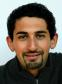
\includegraphics[scale=0.8]{../comon/figures/elias.jpg} } & 24 ans & \textit{Tel:} +41 76 409 0330 \\[0.4cm]
	& Célibataire & \textit{E-mail:} \url{elias.medawar@gmail.com}\\[0.4cm]
  	& Suisse et Libanais\\[0.5cm]
	\end{tabular}
\subsection{Compétences personnelles}
\vspace{-0.4cm}
Passionné, Flexible, Autonome

\subsection{Formation}
\vspace{-0.4cm}
\subsubsection{2008 à aujourd'hui}
\vspace{-0.4cm}
\textbf{Bachelor \textbf{bilingue}(Français-Allemand) en Informatique}\\
\textit{A l'Ecole d'ingénieurs et d'architectes de Fribourg et 1 semestre d'échange à la Hochschule Luzern  }
 \vspace{-0.4cm}
 \subsubsection{2004 à 2008}
 \vspace{-0.4cm}
 \textbf{Maturité professionnelle et apprentissage en Informatique }\\
 \textit{Lycée Technique Baptiste Savoye de St-Imier }
 
\subsection{Informatique}
\vspace{-0.4cm}
\begin{tabular}[t]{lp{5.5cm}l}
 & \textbf{Maitrisé} & \textbf{Connaissances} \\
 Programmation : &  JAVA et JAVA EE, Objective-C(iPhone et iPad) , C\# , PHP, Matlab &  AS3,   C , C++ , VHDL\\ 
 Base de données : &  Oracle , MySQL&  SQL server \\
Méthodologie : & UML & Scrum \\
Bureautique : & Suite office, \LaTeX & \\
\end{tabular}

\subsection{Activités professionnelle et projet  }
\vspace{-0.4cm}
\subsubsection{juin-août 2011}
\vspace{-0.4cm}
\textbf{École supérieure des Ingénieurs de Beyrouth, Liban }Travail de bachelor \\
Création d'une application iPhone/iPad qui permet aux étudiants et professeur de l'université  d'accéder au système d'information de l'école.\\
\textit{Acquis:} Gestion de projet et recherche de solutions innovantes
\vspace{-0.2cm}
\subsubsection{2008 à aujourd'hui}
\vspace{-0.4cm}
\textbf{\href{http://www.misg.ch/}{Multimedia  Information System Group} }Fribourg\\
Collaboration dans différents projets de recherche.
\begin{itemize}
\item \href{http://magisystem.project.eia-fr.ch/}{MAGI System} , test de l'interaction home-machine à l'aide des pensées.
\item \href{http://portal.acm.org/citation.cfm?id=1647363}{WiiNote}, Annotation d'images à l'aide des manettes de la console Wii. 
\end{itemize}
\textit{Acquis:}Autonomie et recherche de solutions innovantes
\vspace{-0.2cm}
 \subsubsection{09/2010 - 02/2011}
 \vspace{-0.4cm}
\textbf{\href{http://www.tura.ch/}{Tura AG, Rotkreuz} }projet de semestre à Luzern\\
Implémentation d'un serveur webDAV en php pour la plateforme  \href{http://www.yaoos.org/}{YaOOS} 
\begin{itemize}
\item Permet le mapage des données comme lecteur réseaux en local
\end{itemize}
\textit{Acquis:}Gestion de projet, analyse des besoins. 
\vspace{-0.2cm}
 \subsubsection{mars - aout 2008}
 \vspace{-0.4cm}
\textbf{\href{http://www.tem-sarl.ch/fr}{Techniques Electroniques Moutier Sàrl}}
\begin{itemize}
\item Création d'un CMS pour la gestion dynamique du  \href{http://www.tem-sarl.ch/fr}{site} de l'entreprise
\end{itemize}
\textit{Acquis:} Rigueur, travail d'équipe 
\vspace{-0.2cm}
 \subsubsection{2006 à 2009}
 \vspace{-0.4cm}
\textbf{Création de sites web en free-lance}\\
\textit{Acquis:}Gestion des priorités, sens de la communication,résistance au stress 

\subsection{Langues }
\vspace{-0.4cm}
Français: Langue maternelle\\
Arabe: Parlé couramment, notions d'écriture  \\
Allemand: Courant (niveau B2-C1 )\\
Anglais: Scolaire (niveau A2), bon vocabulaire technique

\cleardoublepage
%Table of contents page
\thispagestyle{empty}


\begin{spacing}{0.9}
\renewcommand\contentsname{Table des matières}
\tableofcontents
\thispagestyle{empty} 

\end{spacing}

\vspace{1cm}
\begin{large}
\textbf{Évolution de ce  document\\}
\end{large}
\begin{tabular}{|c|l|l|l|}
\hline  Rev &  Date &  Auteur & Remarque \\ 
\hline  1 &  02.06.2011 & Medawar  & Création de la premières version du SRS. \\ 
\hline  2 &  13.06.2011 & Medawar  & Ajouts des éléments pour la release 0.1  . \\ 
\hline  3 &  22.06.2011 & Medawar  & Ajouts des éléments nécessaire pour la release 0.2. \\ 
\hline  4 &  04.07.2011 & Medawar  & Ajouts des éléments nécessaire pour la release 0.3. \\ 

\hline 
\end{tabular} 

\newpage

\cleardoublepage
\chapter{Introduction}
\cleardoublepage
\section{Contexte}
Ce projet s'inscrit dans le cadre du travail de Bachelor pour l'obtention du diplôme de Bachelor à l'Ecole d'ingénieurs et d'architectes de Fribourg. Il est réalisé à l'Université Saint-Joseph au Liban. 

Le potentiel des nouveaux appareils mobiles comme l'iPhone et l'iPad est énorme et il n'est jusqu'à présent pas exploité pour accéder au système d'information de l'\gls{USJ} . A l'aide de ce projet, nous allons exploiter aux mieux les nouvelles technologies et permettre aux utilisateurs du campus de consulter simplement et rapidement des informations telles que le programme des cours, les notes des examens , le plan du campus ou encore l'annuaire du campus.

\section{Structure du rapport}
La documentation du projet a été faite selon la norme IEEE 829-1998 sur la documentation de projet informatique. Cette norme regroupe les informations selon leurs types par documents. 

Dans les équipes de développement d'une grande taille, chaque personne à un rôle dans le projet(Testeur, Architecte, Deseigner,Chef de projet, etc..). La norme permet  en autre de lié le rôle d'un ingénieur à un document.Par exemple le testeur sera responsable du STD(Software Test Documentation), le chef de projet est responsable du SPMP(Software Project Management Plan), etc . Il est claire que dans le cas présent une seul personne travail sur le projet mais grâce à cette manière de documenter,on est obligé de ce mettre dans le rôle de la personne qui est sensé rédiger le document et de ce faite pensé à tout les points importants comme elle le ferait.

Pour une question de lisibilité, les différents documents ont été regroupé sous forme de chapitre pour former le rapport final.\\
Le chapitre~\ref{spmp} à partir de la page \pageref{spmp} regroupe toutes les informations concernant la gestion du projet. En suite vient à partir de la page \pageref{srs} le chapitre~\ref{srs}  qui contient toutes les informations sur l'analyse faite durant le projet. Les pages \pageref{sdd} à \pageref{std} rassemblent toutes la documentation de la conception et implémentation de l'application.  Pour finir vient à la page \pageref{std} tout ce qui concerne les tests et leurs résultats. 
Une conclusion termine le rapport. Elle est suivit par les annexes et information sur le contenu du CD.



\cleardoublepage
\chapter{Software Project Management Plan\label{spmp}}
\vspace{6cm}
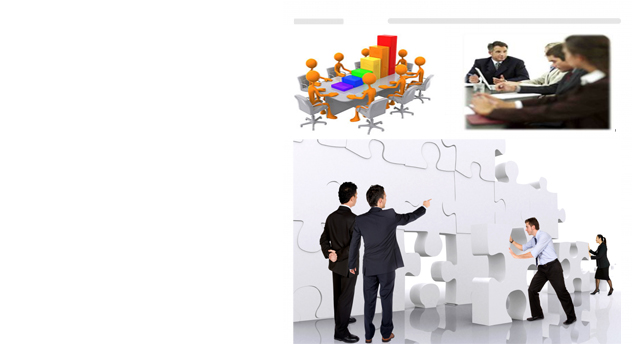
\includegraphics[width=1\textwidth]{../comon/figures/spmpPic.jpg}



\cleardoublepage
	\section{Introduction}
	Ce chapitre regroupe toutes les informations relatives à la gestion du projet et du processus de développement.Ce chapitre est mis à jour régulièrement afin de permettre à tout moment d'avoir un aperçu de l'avancement du projet.

\section{Organisation}
	L'annexe A (/Documentation/Annexes/A\_Directives) contient les directives qui ont été distribuées au début du projet. Ces directives sont la ligne directrice concernant l'organisation du projet et sont complétées par ce document.
	Le cahier des charges de l'annexe G a été créé et validé en début de projet, il est la référence en ce qui concerne les objectifs à atteindre. 
	
	\subsection{Séances}
	\begin{itemize}
		\item Des séances hebdomadaires seront effectuées avec M. Dany Mezher, le responsable externe .
		\item Une séance est tenue si possible toute les 2-3 semaines via Skype avec Mme Mugellini et M. Abou Khaled, les responsables internes.
		\item Au moins une séance est organisée avec les experts M. Roland Marro et M. Marc Wuergler via Skype.
	\end{itemize}
	\subsection{Site internet}
		Un site internet est mis en ligne et il est disponible à l'adresse suivante: \url{https://forge.tic.eia-fr.ch/projects/esibpad} \\
		Mme Mugellini et M. Abou Khaled peuvent utiliser leur login AII pour accéder aux données.\\
		Pour les autres personnes, des comptes ont été créés par le service informatique de l'école. Les comptes sont valides jusqu'au 31.12.2011. \\[1cm]
		
		\begin{table}[H]
			\centering
			\begin{tabular}{|c|c|}
				\hline M.Dany Mezher &  \\ 
				\hline   Username : &  dany.mezher   \\ 
				\hline   Password : & voir mail     \\ [0.2cm]
				\hline M.Marc Wuergler & \\ 
				\hline   Username : &  marc.wuergler  \\ 
				\hline   Password : & voir mail \\ [0.2cm]
				\hline M.Roland Marro &  \\ 
				\hline   Username :&  roland.marro  \\ 
				\hline   Password : & voir mail     \\
				\hline
			\end{tabular} 
			\caption{\label{tab.login}Données de login pour les personnes externe à l'EIA-FR}
		\end{table}
	
		Le site contiendra:
	 	\begin{itemize}
	 		\item le journal de bord :\url{https://forge.tic.eia-fr.ch/projects/esibpad/wiki}
			\item Les PVs :\url{https://forge.tic.eia-fr.ch/projects/esibpad/documents} 
			\item La documentation sous format PDF:\url{https://forge.tic.eia-fr.ch/projects/esibpad/documents} 
		\end{itemize}
	\subsection{Communication}
		Le moyen de communication principal est l'e-mail.\\
		\begin{table}[H]
			\begin{tabular}{|l|l|l|}
				\hline  Nom & email  & Téléphone [Fixe, Mobile]  \\ 
				\hline M. Würgler Marc & marc.wuergler@sunrise.ch  & +41 26 660 03 04, +41 78 609 49 44  \\ 
				\hline M. Marro Roland & marror@fr.ch  & +41 26 305 31 61  \\ 
				\hline M. Dany Mezher	& dany.mezher@fi.usj.edu.lb & +961 142 134 1,+961 700 100 30  \\ 
				\hline Mme Elena Mugellini & elena.mugellini@hefr.ch &  +41 26 429 68 70\\ 
				\hline M. Omar Abou Khaled & omar.aboukhaled@hefr.ch  &  +41 26 429 65 89\\ 
				\hline M. Elias Medawar & elias.medawar@edu.hefr.ch  &  +961 712 900 72, +41 764 090 330\\ 
				\hline 
			\end{tabular} 
			\caption{Résumé des adresses e-mail et des numéros de téléphone.}			
		\end{table}
	
		Des rendez-vous pour des vidéo-conférences seront organisés à l'aide de \gls{Skype}.
\section{Planification}
	\subsection{Plan global}
	 \EPSFIGTEXTWIDTH{../comon/figures/timeLineDetail.pdf}{Vue détaillée du planning du projet}{planGlobDet}

	 \subsection{Description des jalons}

		 \begin{longtable}{|c|l|p{10cm}|}

		 \hline  \textbf{Nom} & \textbf{Date}  & \textbf{But à atteindre}  \\ 
		 \endfirsthead
		  \multicolumn{3}{|r|}{{suite de la page précédente}} \\ \hline
		\hline  \textbf{Nom} & \textbf{Date}  & \textbf{But à atteindre}  \\ 
		 \endhead
		  \multicolumn{3}{|r|}{{Suite à la page suivante}} \\ \hline
		 \endfoot
		 \endlastfoot
		 \hline  Milestone 1 & 03.06.11  & 
		 	\begin{itemize}
		 	 		\item Le cahier des charges est établi et validé.
		 			\item La première version du \gls{SPMP} est rédigée.
		 	\end{itemize}   \\ 
		 \hline  Milestone 2 & 10.06.11  & 
		 	\begin{itemize}
		 	 		\item Pouvoir déployer une simple application sur l'iPhone et l'iPad.
		 			\item Un environnement de développement local est mis en place, avec des Web Services de test ainsi que des données de test.
		 	\end{itemize}   \\ 
	 	 \hline  Release 0.1 & 17.06.11  & 
		 	\begin{itemize}
		 	 		\item La page d'accueil de l'application avec les différents menus est réalisée.
		 			\item La page de paramètres de l'application est réalisée.
		 	\end{itemize}   \\ 
	 	 \hline  Release 0.2 & 01.07.11  & 
		 	\begin{itemize}
		 	 		\item Afficher la carte du campus.
		 	 		\begin{enumerate}[a)]
	 	 				\item La position actuelle de l'utilisateur sera détectée à l'aide du \gls{GPS} de l'appareil et affichée sur la carte.
	 	 				\item L'utilisateur peut, à l'aide de la fonction ''chercher'' : trouver l'emplacement d'une salle ou le bureau d'une personne.
	 	 				\item Les informations de la carte sont enregistrées sur le serveur et peuvent être mises à jour à tout moment. Un système de cache évite de recharger la carte à chaque visite.
	 	 			\end{enumerate}
		 	\end{itemize}   \\ 
		 \hline  Release 0.3 & 13.07.11  & 
 		 	\begin{itemize}
 		 	 		\item Permettre de consulter les nouvelles du campus.
	 		 	 	\begin{enumerate}[a)]
	 		 	 			\item Si une nouvelle est liée à un lieu, permettre de l'afficher facilement sur la carte.
	 		 	 		\end{enumerate}
 		 	\end{itemize}   \\
		\hline  Release 0.4 & 22.07.11  & 
				\begin{itemize}
 		 	 		\item Permettre l'accès à l'annuaire de l'université. 
	 		 	 	\begin{enumerate}[a)]
		 	 				\item Quand on clique sur un numéro de téléphone, l'appel est lancé.
		 	 				\item Quand on clique sur une adresse mail, la fenêtre d'envoi de mail de l'appareil est ouverte.
		 	 			\end{enumerate}
 		 	\end{itemize}   \\
		\hline  Release 0.5 & 03.08.11  & 
 		 
 	 		 	\begin{itemize}
 	 		 	 		\item Permettre aux professeurs et aux étudiants d'afficher leurs horaires.
 		 		 	 	\begin{enumerate}[a)]
 		 		 	 			\item Quand on clique sur un cours, l'emplacement de ce dernier est affiché sur la carte.
 		 		 	 			\item L'utilisateur peut sauvegarder son horaire sur l'appareil pour un accès offline.
 		 		 	 		\end{enumerate}
 	 		 	\end{itemize}   \\ 
	 	\hline  Release 0.6 Version 1 & 03.08.11  & 
 		 	\begin{itemize}
 		 	 		\item Permettre aux étudiants de consulter le résultat des examens. \textbf{Cet objectif est conditionné par l'accord de l'administration et du service informatique de l'\gls{ESIB}.}
 		 	\end{itemize}   \\  
	 	\hline  Milstone 3 &  19.08.11 &
	  		 	\begin{itemize}
	  		 	 		\item L'application est prête à être publiée sur l'App store.
	  		 	 		\item La documentation est finie.
	  		 	 		\item La présentation finale est prête.
	  		 	\end{itemize}   \\  
		 \hline 
		\caption{\label{tab.DescMils}Description des jalons. Les date de releases sont considérées comme des jalons.}  \\
	 \end{longtable} 

	 \begin{landscape}
	 	 \subsection{Planification détaillé}
		 \begin{figure}[H]
			 \begin{center}	
				 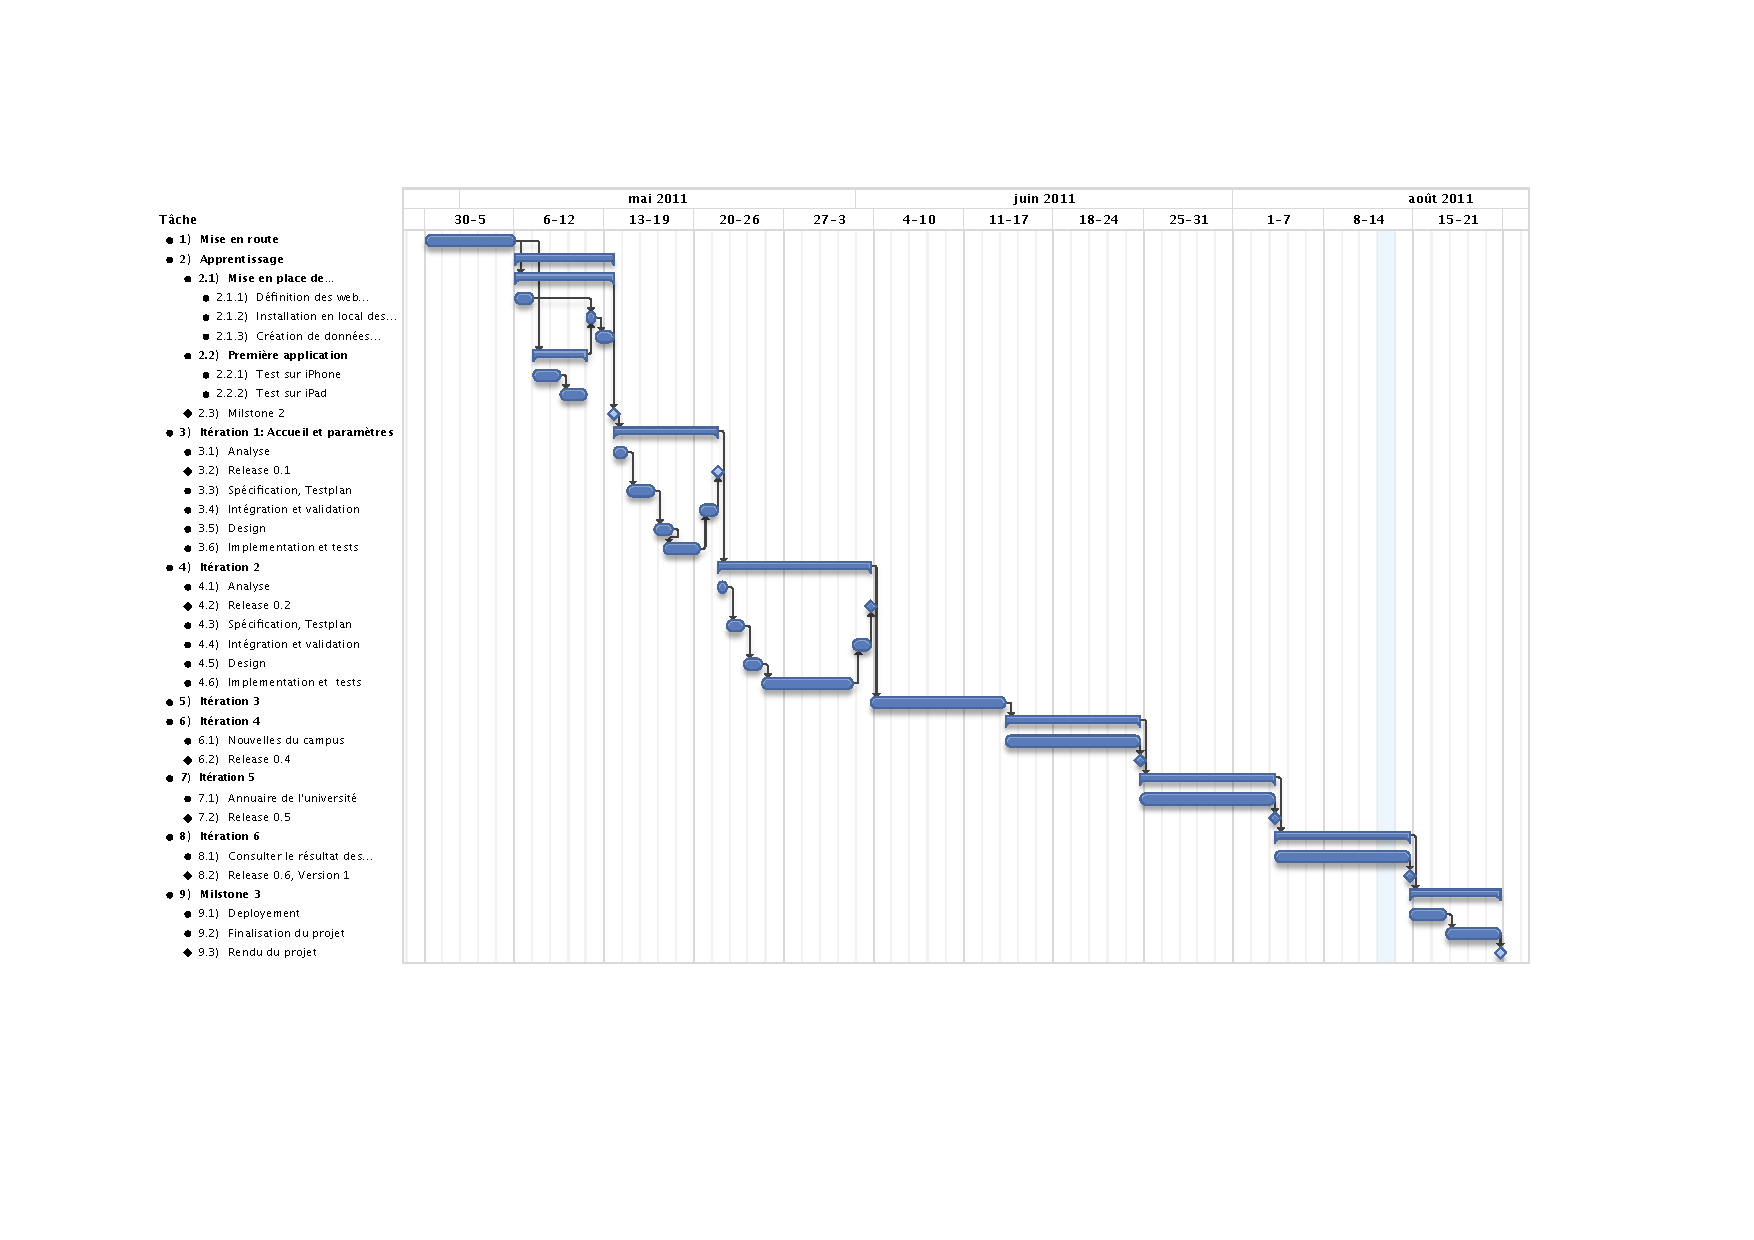
\includegraphics[height=0.8\textwidth]{../comon/figures/planningV3.pdf}
				 \end{center}			
				 \caption{Vue globale du planning du projet avec les milestones}			
				 \label{planV1}			
		 \end{figure}	
	 \end{landscape}
	 La planification détaillée de chaque itération n'est pas  faite, elle sera faite au début de chaque itération si besoin est. Etant seul à travailler sur les tâches et vu que les itérations sont courtes, une planification plus détaillée est inutile. En début d'itération, une liste de tâches à faire (TODO) est faite avec une estimation du temps nécessaire pour atteindre l'objectif. Ce fonctionnement s'approche de la méthode de travail Scrum.
	  
\section{Processus technique}
Sur la Figure~\ref{planGlobDet} nous pouvons voir que nous allons travailler par itérations. Voici une définition plus détaillée de ce que l'on entand par itération 
	 \EPSFIGTEXTWIDTH{../comon/figures/vModel.pdf}{Illustration du modèle de développement en V qui est appliqué à chaque itération. }{vModel}
\textit{``Le modèle du cycle en V a été imaginé pour pallier au problème de réactivité du modèle en cascade. Ce modèle est une amélioration du modèle en cascade qui permet, en cas d'anomalie, de limiter un retour aux étapes précédentes. Les phases de la partie montante doivent renvoyer de l'information sur les phases en vis-à-vis lorsque des défauts sont détectés afin d'améliorer le logiciel.
De plus, le cycle en V met en évidence la nécessité d'anticiper et de préparer dans les étapes descendantes les « attendus » des futures étapes montantes : ainsi les attendus des tests de validation sont définis lors des spécifications, les attendus des tests unitaires sont définis lors de la conception, etc.
Le cycle en V est devenu un standard de l'industrie du développement de logiciel et de la gestion de projet depuis les années 1980. ``}\cite{wikiV}

Ainsi cette approche sera nommée une itération et elle sera répétée à chaque release pour arriver au but qui a été fixé.
\section{Gestion des risques}
Les divers risques qui mèneraient à un échec du projet sont résumés ici. Le but est de mettre à jour les risques régulièrement, et de faire qu'ils diminuent au plus vite. 
	\subsection{État le 01/06/2011  }
	\begin{table}[H]
	\begin{tabular}{|l|p{6cm}|l|l|l|p{6cm}|}
		\hline  Nr. & Risque & P  & DC & I & Mesure \\ 
		\hline  T1 & Le peu d'expérience dans le développement \gls{Objective-C} induit en erreur(sous estimation de la charge de travail, mauvaise architecture,etc) lors de la prise de décisions importantes au début du projet & 3 & 3 & 9 & Discuter les décisions avec des personnes ayant de l'expérience dans le domaine, prendre le temps d'apprendre les bases de l'\gls{Objective-C} au début du projet et prévoir une tâche simple pour la première itération.  \\ 
		\hline  T2 & Les services web ne sont pas encore opérationnels et peuvent retarder l'avancement du projet & 3 & 3 & 9 & Prévoir un environnement de développement en local avec des Web Services de test indépendants.  \\ 
		\hline  N1 & La méthodologie de travail au sein de l' \gls{EIA-FR} diffèrent trop de celle de l'\gls{ESIB}  et les méthodes ne conviennent pas à l'une ou l'autre partie.  & 1 & 2 & 2 & Organiser régulièrement des séances pour valider les décisions.  \\ 
		\hline  N2 & Sous-estimation de la charges de travail, dépassement du temps mis à disposition.  & 2 & 2 & 4 & Travailler par itération et se baser sur l'expérience acquise lors des itérations précédentes pour bien planifier les suivantes.Ne pas rester bloqué sur une étape sans demander de l'aide.  \\ 
		
		\hline 
	\end{tabular} 
	\caption{ Risques identifié au lancement du projet.\\ Légende :\\
Tx = Risque technique\\
Nx = Risque non technique\\
P = Probabilité  (1 peu probable / 3 très probable)\\ 
DC = Dégât et conséquence (1 peu / 3 grave)\\
I =  Importance ([1-2 petite][3-4 moyenne][5-9 sérieux])(P*DC)
}
	\end{table}
Les risques T1 et T2 qui sont d'une grande importance ont été pris en considération pour la planification.
	\subsection{État le 04/07/2011  }
	\begin{table}[H]
	\begin{tabular}{|l|p{6cm}|l|l|l|p{6cm}|}
		\hline  Nr. & Risque & P  & DC & I & Mesure \\ 
		\hline  {\color{green}T1} & Le peu d'expérience dans le développement \gls{Objective-C} induit en erreur(sous estimation de la charge de travail, mauvaise architecture,etc) lors de la prise de décisions importantes au début du projet & 2 & 3 & 6 & Ce risque à diminuer suite à l'expérience acquise durant la première itération.  \\ 
		\hline  {\color{green}T2} & Les Web Services ne sont pas encore opérationnels et peuvent retarder l'avancement du projet & 1 & 3 & 3 & Diminution suite à la création d'un environnement de test stable et contrôlable. Une première version des web services a été mis en place par le service informatique de l'\gls{USJ}  .  \\ 
		\hline  N1 & La méthodologie de travail au sein de l' \gls{EIA-FR} diffèrent trop de celle de l'\gls{ESIB}  et les méthodes ne conviennent pas à l'une ou l'autre partie.  & 1 & 2 & 2 & Organiser régulièrement des séances pour valider les décisions.  \\ 
		\hline  {\color{red}N2} & Sous-estimation de la charges de travail, dépassement du temps mis à disposition.  & 3 & 2 & 6 & Suite au retard pris lors de la première itération ce risque augmente.  \\ 
		
		\hline 
	\end{tabular} 
	\caption{ Risques après la première itération.\\ Légende :\\
Tx = Risque technique\\
Nx = Risque non technique\\
P = Probabilité  (1 peu probable / 3 très probable)\\ 
DC = Dégât et conséquence (1 peu / 3 grave)\\
I =  Importance ([1-2 petite][3-4 moyenne][5-9 sérieux])(P*DC)
}
	\end{table}
Les probabilités des risques T1 et T2  ont diminué après le premier mois de développement tandis que celle du risque N2 a augmenté. On peut constater que globalement les risques diminuent. Il faut travailler sur la planification pour diminuer au plus vite le risque N2.

	\subsection{État le 08/08/2011  }
	\begin{table}[H]
	\begin{tabular}{|l|p{6cm}|l|l|l|p{6cm}|}
		\hline  Nr. & Risque & P  & DC & I & Mesure \\ 
		\hline  {\color{green}T1} & Le peu d'expérience dans le développement \gls{Objective-C} induit en erreur(sous estimation de la charge de travail, mauvaise architecture,etc) lors de la prise de décisions importantes au début du projet &0 & 3 & 0 & Ce risque peut être considéré nul vu l'expérience acquise jusq'à présent   \\ 
		\hline  {\color{green}T2} & Les Web Services ne sont pas encore opérationnels et peuvent retarder l'avancement du projet & 1 & 1 & 1 & aucun changement.  \\ 
		\hline  \color{green}N1 & La méthodologie de travail au sein de l' \gls{EIA-FR} diffèrent trop de celle de l'\gls{ESIB}  et les méthodes ne conviennent pas à l'une ou l'autre partie.  & 0 & 2 & 0 & Le système des 2 écoles n'est pas incompatibles et la manière de travail convient aux 2 selon les différentes séance organisées et les commentaires émis. .  \\ 
		\hline  {\color{green}N2} & Sous-estimation de la charges de travail, dépassement du temps mis à disposition.  & 1 & 2 & 2 & Des heures de travail supplémentaires ont été faites pour rattraper le retard et on est dans le temps selon la planification.  \\ 
		\hline 
	\end{tabular} 
	\caption{ Risques après la première itération.\\ Légende :\\
Tx = Risque technique\\
Nx = Risque non technique\\
P = Probabilité  (1 peu probable / 3 très probable)\\ 
DC = Dégât et conséquence (1 peu / 3 grave)\\
I =  Importance ([1-2 petite][3-4 moyenne][5-9 sérieux])(P*DC)
}
	\end{table}
A cette étape du projet, on peut dire que les risques d'échec sont quasi nuls, il faut toutefois garder un rythme de travail assez soutenu pour parvenir au bout à temps.  

\section{Gestion des configurations}
Afin de garder des traces de l'évolution du projet, des versions des sources des documents seront sauvegardées sur un serveur \gls{SVN}. La version courante du projet est hébergée à l'adresse suivante:  \sout{\url{http://esibpad.googlecode.com/svn/trunk/}} \url{https://github.com/eia-fr/ESIB_PAD/}\footnote{Suite à des problèmes technique rencontré pour communiquer via SVN, le protocole \gls{Git} est utilisé à partir de la release 2} . Les releases seront stockées  à l'emplacement suivant: \sout{\url{http://esibpad.googlecode.com/svn/tags/}} \url{ https://github.com/eia-fr/ESIB_PAD/tree/} 

	 \EPSFIGTEXTWIDTH{../comon/figures/config0_5}{Compatibilité entre composants et versions du logiciel. Les traits continus représentent une compatibilité à 100 \%, les traits traitillés représentent une compatibilité partielle.}{config0_5}
	 
\textbf{GCCalendar} : est un composant externe open source qui permet d'afficher un calendrier pour une journée.\cite{gcCalendar} La version  v 1.1.1 est une adaptation de la version officielle faite par moi-même pour mieux répondre aux besoins du projet et qui permet l'affichage du composant dans une partie de l'écran pour l'iPAD et non uniquement en plein écran sur iPhone.Cette adaptation prend aussi en charge le changement de journée grâce au mouvement ''glisser'' du doigt sur l'écran. Cette version a été transmise à l'auteur pour ainsi faire évoluer ce composant.

\section{Gestion de la documentation}
 La documentation sera conçue selon les différentes normes IEEE sur la documentation de software. Elle contiendra notamment les documents suivants:

\begin{enumerate}
	\item \gls{SPMP} - Software Project Management Plan (IEEE 1058).  Ce document contient toutes les informations concernant l'organisation d'un projet de développement de software . Il a pour but de rendre transparente l'organisation du projet et aide les chefs de projets à avoir un aperçu global de l'état d'avancement.
	\item \gls{SRS} - Software Requirements Specification(IEEE 830). Ce document contient la documentation concernant la spécification et l'analyse.
	\item \gls{SDD} - Software Design Description(IEEE 1016). Ce document contient la documentation concernant la conception  et l'implémentation.
	\item \gls{STD} - Software Test Documentation(IEEE 1008). Ce document contient la documentation concernant les tests effectués.
\end{enumerate}	

Il est important d'indiquer que la documentation ne sera pas complètement conforme à la norme, car cela représenterait une trop grande charge de travail. En effet, les différentes normes sont très complètes et plusieurs chapitres ne sont pas adaptés à notre projet. La variante de documentation qu'on utilise est inspirée de celle utilisé par la ''Hochschule Luzern '' (école d'ingénieurs Suisse alémanique dans laquelle j'ai eu l'occasion d'étudier durant 6 mois).

Les documents seront regroupés en chapitre pour former le rapport final du projet.

\section{Gestion des finances}
Ce travail fait partie du processus de formation et ne traite pas en détail de l'aspect financier. Cependant voici tout de même quelques informations que l'on peut citer:
\subsection{Ressources humaines}
\begin{itemize}
	\item 1 futur ingénieur HES  à 100\%  soit 40 heures par semaine durant 12 semaines. Une bourse est versée par  l'\gls{EIA-FR} à l'étudiant pour le transport jusqu'au Liban ainsi que le logement sur place. 
\end{itemize}
\subsection{Ressources matérielles}
\begin{itemize}
	\item 1 iPad2 et 1 iPhone 4  mis à disposition par l'\gls{EIA-FR}
	\item local de travail mis à disposition par l'\gls{ESIB}
\end{itemize}

\cleardoublepage
\chapter{Software Requirement Specification\label{srs}}
\vspace{6cm}
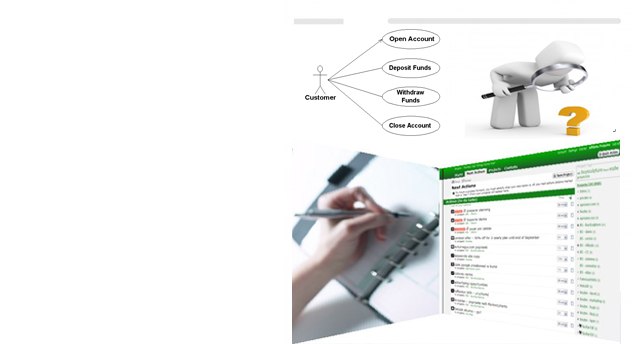
\includegraphics[width=1\textwidth]{../comon/figures/srsPic.jpg}
\cleardoublepage
\section{Introduction}
Ce chapitre contient les spécifications détaillées des exigences du projet ainsi que l'analyse faite pour chaque tâche. Ces deux étapes sont essentielles pour partir dans la bonne direction dès le début de chaque itération.  La section analyse décrit en général les cas d'utilisation que l'on identifie ainsi que la faisabilité de ces derniers. Le détail des cas d'utilisation et de leurs besoins graphique est documenté dans la section exigences fonctionnelles de ce chapitre.
\section{Analyse}
	\subsection{ Aperçu global}
	 \EPSFIGTEXTWIDTH{../comon/figures/apercu.pdf}{Vue globale des fonctionnalités du produit}{apercuGlob}
	\subsection{Use case}
	 \EPSFIGTEXTWIDTH{../comon/figures/UC.pdf}{Diagramme des cas d'utilisation de l'application}{UC}
	 Les fiches descriptives du chapitre~\ref{exigenceFoction} détaillent les cas d'utilisation.
	\subsection{Description des utilisateurs}
		\textbf{Professeurs :} représente les professeurs de l'USJ.\\[0.2cm]
		\textbf{Étudiants :} représente les étudiants de l'USJ.\\[0.2cm]
		\textbf{Visiteurs :} représente les visiteurs et les personnes non enregistrées de l'USJ.\\[0.2cm]
		\textbf{WebServices :} représente les web services de l'\gls{USJ} qui nous permettent d'accéder aux informations de la base de données.\\[0.2cm]
		\textbf{FS\_Local :} représente les données stockées en local sur l'appareil.\\[0.2cm]
		\textbf{BD Google map :} représente la base de données Google pour les images de la carte.\\[0.2cm]
		
	\subsection{Faisabilité}
		\textbf{UC\_0  Naviguer}  L'\gls{iOS} permet d'afficher différentes vues et naviguer d'une façon simple entre elles. Ce cas d'utilisation est \textbf{100 \%  faisable}.\\[0.2cm]
		\textbf{UC\_1  Paramétrage}  L'\gls{iOS} permet de stocker des paramètres d'application d'une façon simple. Ce cas d'utilisation est \textbf{100 \%  faisable}.\\[0.2cm]
		\textbf{UC\_3  Carte}  La librairie MapKit livrée avec l'\gls{iOS} permet d'afficher des cartes en se basant sur la base de données de google map.Il est aussi possible d'ajouter des annotations à des emplacement précis de la carte. Cette librairie est utilisable gratuitement et librement, elle répond à tous les besoins de notre application.Il est aussi possible, grâce au gps des appareils, de détecter la position de l'utilisateur.  Ce cas d'utilisation est \textbf{100 \%  faisable}.\\[0.2cm]
		\textbf{UC\_4  AfficherNews}  Les outils à disposition permettent d'effectuer aisément ce genre de tâches . Pour le détail des news, il est possible d'intégrer un navigateur web dans l'application. Ce cas d'utilisation est \textbf{100 \%  faisable}.\\[0.2cm]
		\textbf{UC\_5 AfficherAnnuaire}  L'annuaire est disponible via les web services, le but ici est de le présenter d'une façon pratique à l'utilisateur. Ce cas d'utilisation est \textbf{100 \%  faisable}.\\[0.2cm]
		\textbf{UC\_6 AfficherHoraire}  L'annuaire n'est pas disponible via les web services, les données seront simulées à l'aide du web service local	sur la machine du développeur. \textbf{80 \%  faisable}.\\[0.2cm]
		\textbf{UC\_7 AfficherNoteExamen}   Les notes d'examens ne sont pas disponibles via les web services, les données seront simulées à l'aide du web service local sur la machine du développeur. \textbf{80 \%  faisable}.\\[0.2cm]
		
\section{Spécification des exigences }
	\subsection{Spécification des interfaces}
		\textbf{Interfaces utilisateur}  
			Aucune ligne graphique n'est imposée, la seule contrainte est d'utiliser les logos originaux de l'école.\\[0.2cm]
		\textbf{Interfaces Hardware} 
			L'iPhone et l'iPad possèdent un écran tactile qui sera utilisé pour interagir avec l'utilisateur. D'autres capteurs comme le gyroscope,caméra ou accéléromètre sont disponibles sur l'appareil mais ne seront pas utilisés pour ce projet. \\
			L'iPhone et l'iPad se connectent à internet via le 3Gs et le WIFI pour récupérer les données des web services.\\[0.2cm]
	 	\textbf{Interfaces Software} 
			L'application utilise les web services de l'\gls{USJ} pour accéder aux bases de données. Les web services n'existant pas avant la création de l'application, il faut définir la manière de communiquer avec les web services. Pour ce faire, M.Medawar fournit un fichier XML ainsi que le XML Schema correspondant au résultat attendu d'un web service et le service informatique de l'USJ fournira ce service.  L'annexe E(/Documentation/Annexes/E) contient tout les fichiers XML et XML Schema fournis au service informatique. \\

			  \begin{lstlisting}[language=XML,caption = Exemple de code XML fournit au service informatique de l'USJ]
<?xml version="1.0" encoding="UTF-8"?>
<!-- Resultat de l'appel https://www.url.com/webSerivice.php 
    avec les parametres en POST suivant:
    usr = 'elias.medawar'
    pwd = '1234'
    op  = 'testCommunication'
-->
<response xmlns:xsi="http://www.w3.org/2001/XMLSchema-instance"
 xsi:noNamespaceSchemaLocation="schemaTest.xsd">
    <!-- Une reponse valide pour tester la communication -->
    <status>0</status>
    <usrGroup>2</usrGroup>
    <commentaire><![CDATA[Communication possible]]></commentaire>
</response>
			\end{lstlisting}

 \begin{lstlisting}[language=XSD,caption = Exemple de XML Schema fournit au service informatique de l'USJ]
<?xml version="1.0" encoding="UTF-8"?>
<xs:schema xmlns:xs="http://www.w3.org/2001/XMLSchema" elementFormDefault="qualified">
  <xs:element name="response">
    <xs:complexType>
      <xs:sequence>
        <xs:element ref="status"/>
        <xs:element ref="usrGroup"/>
        <xs:element ref="commentaire" minOccurs="0" maxOccurs="10"/>
      </xs:sequence>
    </xs:complexType>
  </xs:element>
  <xs:element name="status">
    <xs:simpleType>
      <xs:restriction base="xs:int">
        <xs:enumeration value="-2"></xs:enumeration><!-- Intenrnal error in the webservices.KO -->
        <xs:enumeration value="-1"></xs:enumeration><!-- Wrong password or login.KO -->
        <xs:enumeration value="0"></xs:enumeration><!-- Successful execution.OK -->
      </xs:restriction>
    </xs:simpleType>
  </xs:element>
  <xs:element name="usrGroup">
    <xs:simpleType>
      <xs:restriction base="xs:int">
        <xs:enumeration value="0"></xs:enumeration><!-- User login is not a registred, asume that it's a visitor -->
        <xs:enumeration value="1"></xs:enumeration><!-- User login correspond to a professor -->
        <xs:enumeration value="2"></xs:enumeration><!-- User login correspond to a student -->
      </xs:restriction>
    </xs:simpleType>
  </xs:element>
  <xs:element name="commentaire" type="xs:string"/>
</xs:schema>
			\end{lstlisting}
	Les fichiers XML ainsi que leur format n'ont pas été pris en compte lors du développement des webservices. Le service informatique a décidé d'utiliser son propre format. Donc les fichiers XML fournis ont simplement été ignorés et ne sont pas à exploiter.\\
	\textbf{Protocoles de communications:} L'application communique officiellement via HTTPS avec les web services, mais pour l'instant les services web sont configurés pour communiquer via HTTP. \\[0.2cm]
	
	
	
	\subsection{Exigences fonctionnelles \label{exigenceFoction}}
		Pour définir correctement les exigences, la description des cas d'utilisation est effectuée. Des prototypes de l'interface graphique sont aussi réalisés. Ces prototypes sont utilisés comme documents de travail lors la prise de décision concernant l'emplacement des éléments et leurs fonctionnements. Ce concept et cette manière de travailler sont inspirés de diverses références bibliographiques à ce sujet\cite{bookErgo}.   Certains prototypes ne représentent pas toujours la version finale implémentée car la version finale est implémentée en fonction des possibilités du système et du temps à disposition . 
		
		Les prototypes ont été faits au départ en version informatique mais par la suite ils ont été fait à la main pour une question de gain de temps. Les prototypes faits à la main ont été remplacés dans la documentation par des captures d'écran qui correspondent.
		 
		\subsubsection{Naviguer}
				L'utilisateur doit pouvoir naviguer dans les différents menus de l'application.\\[0.2cm]
				\begin{longtable}{|l|p{10cm}|}
					\hline \textbf{Nom du Use Case} & Naviguer \\ 
					\hline \textbf{Ref} & UC\_0  \\ 
					\hline \textbf{Déclencheur} & L'utilisateur démarre l'application \\
					\hline \textbf{Précondition} &  \\
					\hline \textbf{Scénario nominal} & 
					\begin{enumerate}
						\item Le système affiche le menu de l'application.
						\item L'utilisateur clique sur  un élément du menu.
						\item Le système affiche la vue correspondante au bouton cliqué .
						\item L'utilisateur effectue la tâche dont il a besoin à l'aide de la vue affichée.
						\item L'utilisateur revient sur la page du menu de l'application.
						\item Recommencement au point 2 du UC.
					\end{enumerate}
					\\ 
					\hline \textbf{Enchaînements alternatifs} &  
						Commence au point 4 du scénario nominal(sur IPad).
						\begin{enumerate}
							\item L'utilisateur clique sur un autre élément du menu.
							\item Continue au point 3 du scénario nominal.
						\end{enumerate}
						
					\\
					\hline \textbf{Status actuel} & Planifié:\CheckedBox , Implémenté:\CheckedBox , Testé: \CheckedBox , Validé: \CheckedBox \\
					\hline 
				\end{longtable} 
		\subsubsection*{Besoin graphique}
				\begin{figure} [H]
					\centering 
					\subfigure[Navigation sur IPhone]{\label{MainMenuIPhone}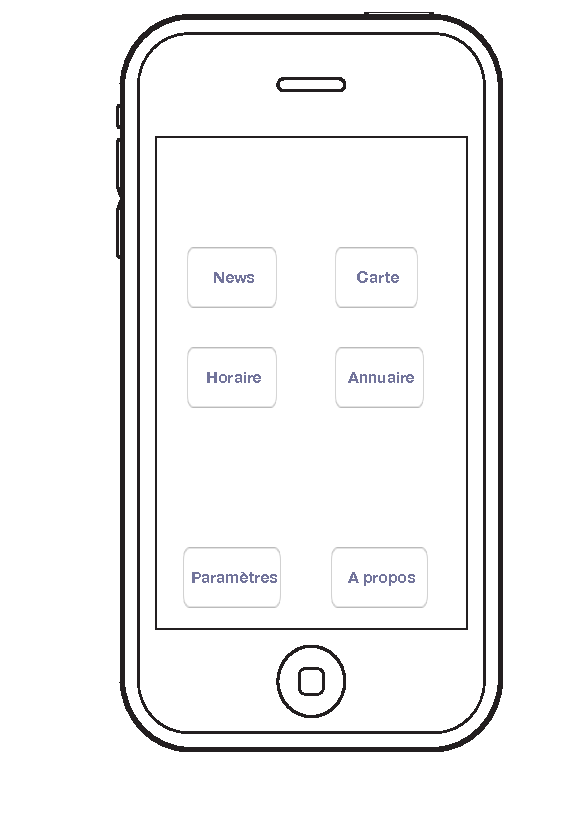
\includegraphics[width=0.3\textwidth]{../comon/figures/MainMenuIPhone.pdf}} 
					\subfigure[Navigation sur IPad]{\label{MainMenuIPad}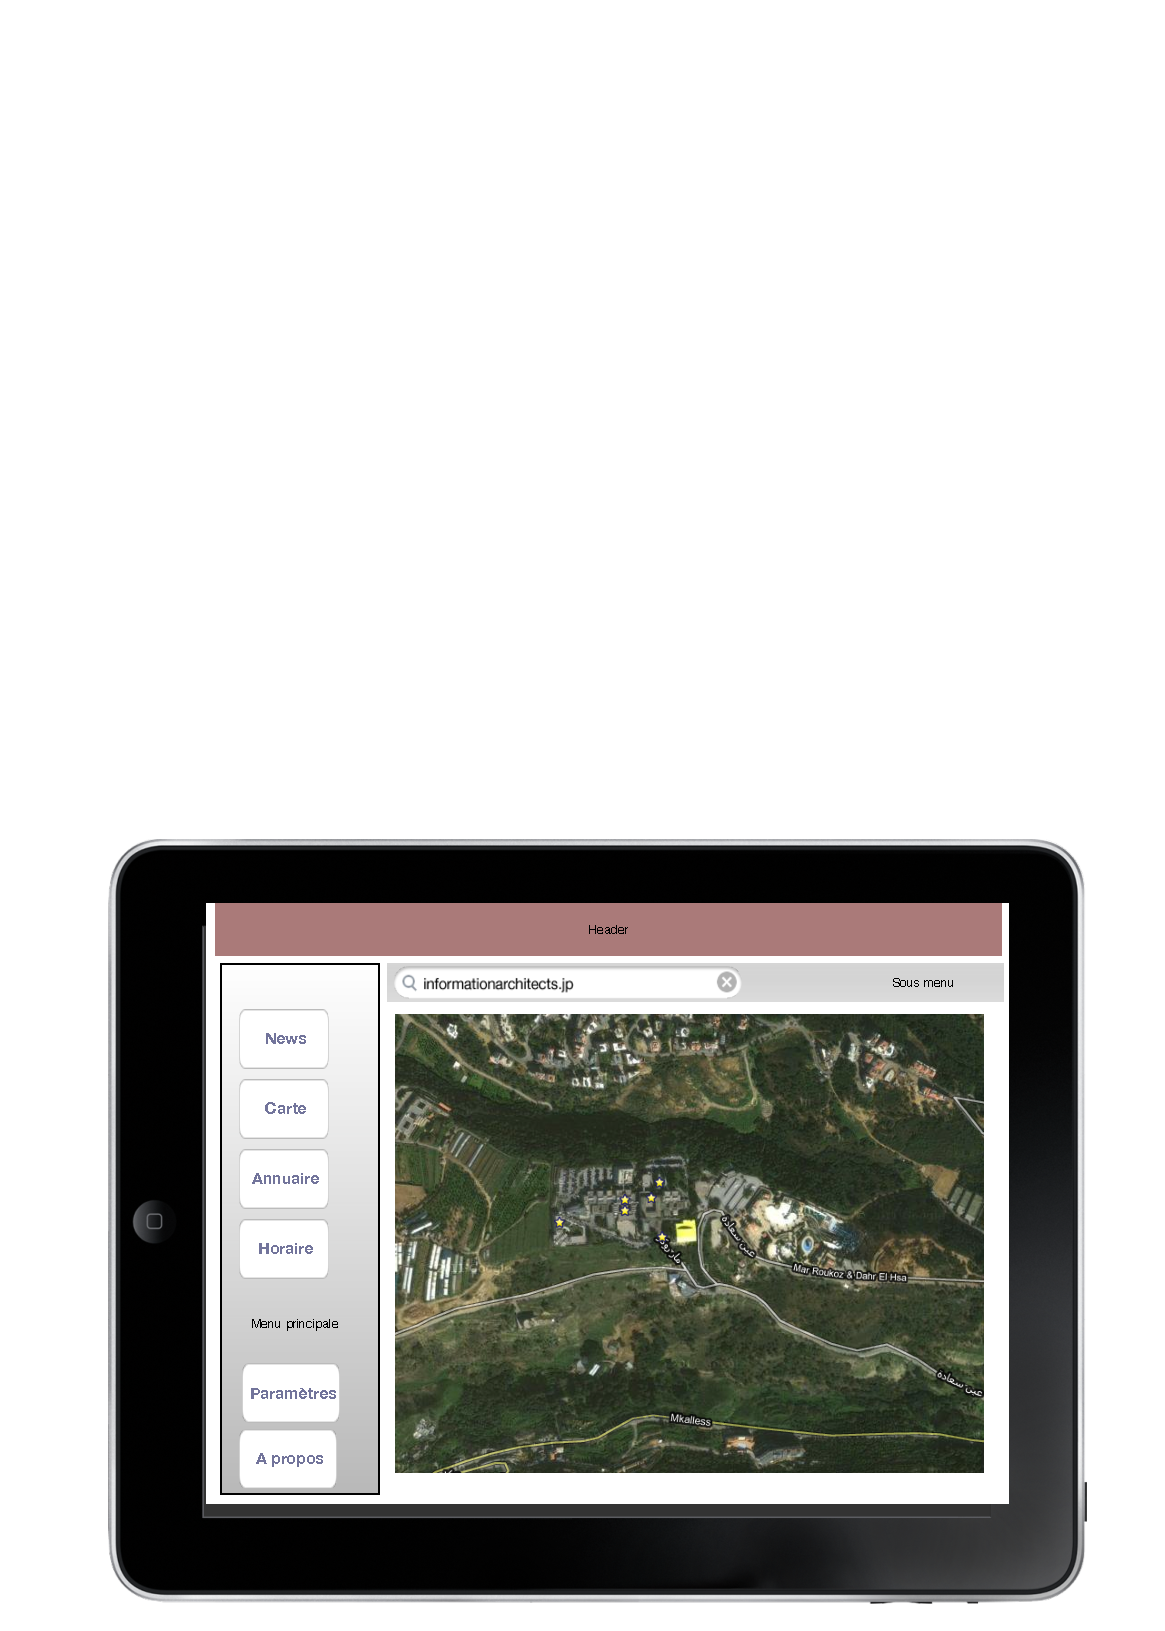
\includegraphics[width=0.6\textwidth]{../comon/figures/MainMenuIPad.pdf}} 
				\end{figure}
				
				
				
		\subsubsection{Paramétrer l'application}
			L'utilisateur doit pouvoir choisir les paramètres de l'application et les sauvegarder.\\[0.2cm]
			\begin{longtable}{|l|p{10cm}|}
				\hline \textbf{Nom du Use Case} & Paramétrage \\ 
				\hline \textbf{Ref} & UC\_1  \\ 
				\hline \textbf{Déclencheur} & L'utilisateur clique sur le bouton paramètre de la navigation\\
				\hline \textbf{Précondition} &  \\
				\hline \textbf{Scénario nominal} & 
				\begin{enumerate}
					\item Le système restaure les valeurs des paramètres depuis le fichier de configuration et les affiche.
					\item L'utilisateur choisit une option qu'il désire modifier.
					\item L'utilisateur modifie la valeur.
					\item \label{uc1Mod}L'utilisateur confirme qu'il a finit de modifier la valeur
					\item Le système sauvegarde la valeur.
				\end{enumerate}
				\\ 
				\hline \textbf{Enchaînements alternatifs} &  \\
				\hline \textbf{Status actuel} & Planifié:\CheckedBox , Implémenté:\CheckedBox , Testé: \CheckedBox , Validé: \CheckedBox \\
				\hline 
			\end{longtable} 
		\subsubsection*{Besoin graphique}
		\EPSFIGTEXTWIDTH{../comon/figures/WierframeIPhoneSettings.pdf}{Wireframe illustrant les modifications des paramètres sur l'iPhone}{WierframeIPhoneSettings}
		
		\EPSFIGTEXTWIDTH{../comon/figures/WierframeIPadSettings.pdf}{Wireframe illustrant les modifications des paramètres sur l'iPad}{WierframeIPadSettings}


		\subsubsection{Visualiser la carte}
					L'utilisateur doit pouvoir visualiser la carte du campus avec les différentes informations utiles pour se retrouver dans le campus.\\[0.2cm]
					\begin{longtable}{|l|p{10cm}|}
						\hline \textbf{Nom du Use Case} & Carte \\ 
						\hline \textbf{Ref} & UC\_3  \\ 
						\hline \textbf{Déclencheur} & L'utilisateur presse sur le bouton carte de l'application \\
						\hline \textbf{Précondition} &  \\
						\hline \textbf{Scénario nominal} & 
						\begin{enumerate}
							\item Le système affiche la carte de tous les campus ainsi que la position actuelle de l'utilisateur.
							\item Le système permet de choisir un campus pour en voir le détail.
							\item Le système affiche les bâtiments principaux du campus.
							\item Le système permet de naviguer, sélectionner des bâtiments ou une personne pour les afficher sur la carte.
						\end{enumerate}
						\\ 
						\hline \textbf{Enchaînements alternatifs} & \\
						\hline \textbf{Status actuel} & Planifié:\CheckedBox , Implémenté:\CheckedBox  , Testé: \CheckedBox  , Validé: \CheckedBox  \\
						\hline 
					\end{longtable} 
			\subsubsection*{Besoin graphique}
					\EPSFIGTEXTWIDTH{../comon/figures/MapIPhone.pdf}{Wireframe illustrant les fenêtres de l'affichage des cartes sur l'iPone}{MapIPhone}

					\EPSFIGTEXTWIDTH{../comon/figures/MapIPad.pdf}{Wireframe illustrant les fenêtres de l'affichage des cartes sur l'iPad}{MapIPad}
					Sur la Figure~\ref{MapIPad} on peut voir, que les menus des deux versions sont les mêmes mais sur l'iPad, au lieu d'ouvrir chaque élément du menu dans une nouvelle fenêtre, les éléments sont ajouté comme des ''Pop-up'' dans la page principale.

	\subsubsection{Afficher les nouvelles}
					L'utilisateur doit pouvoir visualiser les nouvelles du campus .\\[0.2cm]
					\begin{longtable}{|l|p{10cm}|}
						\hline \textbf{Nom du Use Case} & AfficherNews \\ 
						\hline \textbf{Ref} & UC\_4  \\ 
						\hline \textbf{Déclencheur} & L'utilisateur presse sur le bouton news de l'application \\
						\hline \textbf{Précondition} &  \\
						\hline \textbf{Scénario nominal} & 
						\begin{enumerate}
							\item Le système affiche les news du campus.
							\item L'utilisateur peut cliquer sur une news pour voir le détail de cette dernière.
							\item Depuis le détail de la news, l'utilisateur peut, à l'aide d'un bouton retour, revenir à l'aperçu de l'ensemble des news.
						\end{enumerate}
						\\ 
						\hline \textbf{Enchaînements alternatifs} & \\
						\hline \textbf{Status actuel} & Planifié:\CheckedBox , Implémenté:\CheckedBox  , Testé: \CheckedBox  , Validé: \CheckedBox  \\
						\hline 
					\end{longtable} 
			\subsubsection*{Besoin graphique}
					\EPSFIGTEXTWIDTH{../comon/figures/WierframeIPhoneNews.pdf}{Wireframe illustrant les fenêtres de l'affichage des news sur l'iPone}{WierframeIPhoneNews}

					\EPSFIGTEXTWIDTH{../comon/figures/WierframeIPadNews.pdf}{Wireframe illustrant les fenêtres de l'affichage des news sur l'iPad}{WierframeIPadNews}


			\subsubsection{Afficher l'annuaire}
					L'utilisateur doit pouvoir visualiser l'annuaire de l'USJ.\\[0.2cm]
					\begin{longtable}{|l|p{10cm}|}
						\hline \textbf{Nom du Use Case} & AfficherAnnuaire \\ 
						\hline \textbf{Ref} & UC\_5  \\ 
						\hline \textbf{Déclencheur} & L'utilisateur presse sur le bouton annuaire  de l'application \\
						\hline \textbf{Précondition} &  \\
						\hline \textbf{Scénario nominal} & 
						\begin{enumerate}
							\item Le système affiche la liste des possibilités de regroupement:
								\begin{enumerate}
									\item Par campus
									\item Par institution
									\item Services
								\end{enumerate}
							\item L'utilisateur choisit un regroupement qu'il veut
							\item L'utilisateur choisit le sous-groupe désiré.
							\item Le système cherche les données en cache si elles s'y trouvent sinon depuis les services web.
							\item Le système affiche la liste des personnes trouvées.
							\item L'utilisateur presse sur le bouton pour obtenir plus de détail d'une personne.
							\item Le système affiche le détail de la personne.
							\item Le système permet le démarrage d'appel sur un clique sur le numéro de téléphone ou l'envoi d'un e-mail suite à un clique sur l'adresse mail.
						\end{enumerate}
						\\ 
						\hline \textbf{Enchaînements alternatifs} & \\
						\hline \textbf{Status actuel} & Planifié:\CheckedBox , Implémenté:\CheckedBox  , Testé: \CheckedBox  , Validé: \CheckedBox  \\
						\hline 
					\end{longtable} 
			\subsubsection*{Besoin graphique}
					\EPSFIGTEXTWIDTH{../comon/figures/WierframeIPhoneDirectory.pdf}{Wireframe illustrant les fenêtres de l'affichage de l'annuaire sur l'iPone}{WierframeIPhoneDirectory}

					\EPSFIGTEXTWIDTH{../comon/figures/WierframeIPadDirectory.pdf}{Wireframe illustrant les fenêtres de l'affichage de l'annuaire sur l'iPad}{WierframeIPadDirectory}


			\subsubsection{Afficher l'horaire}
								Les utilisateurs de l'USJ  doivent pouvoir visualiser leurs horaires.\\[0.2cm]
								\begin{longtable}{|l|p{10cm}|}
									\hline \textbf{Nom du Use Case} & AfficherHoraire \\ 
									\hline \textbf{Ref} & UC\_6  \\ 
									\hline \textbf{Déclencheur} & L'utilisateur presse sur le bouton horaire de l'application \\
									\hline \textbf{Précondition} &  \\
									\hline \textbf{Scénario nominal} & 
									\begin{enumerate}
										\item Le système affiche un calendrier contenant le jour courant. 
										\item L'utilisateur peut naviguer facilement au jours suivants et précédents. 
										\item L'utilisateur peut, en cliquant sur un cours, afficher son emplacement.
									\end{enumerate}
									\\ 
									\hline \textbf{Enchaînements alternatifs} & \\
									\hline \textbf{Status actuel} & Planifié:\CheckedBox , Implémenté:\CheckedBox  , Testé: \CheckedBox  , Validé: \CheckedBox	  \\
									\hline 
								\end{longtable} 
						\subsubsection*{Besoin graphique}
								\EPSFIGTEXTWIDTH{../comon/figures/wireframeHorraireIPhone.pdf}{Wireframe illustrant les fenêtres de l'horaire sur l'iPone}{WierframeIPhoneNews}
			
								\EPSFIGTEXTWIDTH{../comon/figures/wireframeHorraireIPad.pdf}{Wireframe illustrant les fenêtres de l'horaire sur l'iPad}{WierframeIPadNews}
								

			\subsubsection{Afficher le résultat des examens}
								Les étudiants de l'USJ doivent pouvoir visualiser leurs résultats d'examen.\\[0.2cm]
								\begin{longtable}{|l|p{10cm}|}
									\hline \textbf{Nom du Use Case} & AfficherNoteExamen \\ 
									\hline \textbf{Ref} & UC\_7  \\ 
									\hline \textbf{Déclencheur} & L'utilisateur presse sur le bouton résultat d'examen de l'application \\
									\hline \textbf{Précondition} &  \\
									\hline \textbf{Scénario nominal} & 
									\begin{enumerate}
										\item Le système affiche la liste des examens et la note obtenue. 
									\end{enumerate}
									\\ 
									\hline \textbf{Enchaînements alternatifs} & 
										Commence au point 0 du scénario  nominal quand l'utilisateur n'est pas un étudiant.
									\begin{enumerate}
										\item Le système affiche un message d'erreur.
										\item Le système redirige l'utilisateur vers la fenêtre de paramétrage de l'application.
									\end{enumerate}\\
									\hline \textbf{Status actuel} & Planifié:\CheckedBox , Implémenté:\CheckedBox  , Testé: \CheckedBox  , Validé: \CheckedBox	  \\
									\hline 
								\end{longtable} 
						\subsubsection*{Besoin graphique}
								\EPSFIGSCALE[1.5]{../comon/figures/wireframeNoteIPhone.pdf}{Wireframe illustrant les fenêtres des résultats d'examen sur l'iPone}{WierframeIPhoneNews}
			
								\EPSFIGSCALE[1.5]{../comon/figures/wireframeNoteIPad.pdf}{Wireframe illustrant les fenêtres des résultats d'examen sur l'iPad}{WierframeIPadNews}

\cleardoublepage
\chapter{Software Design Description\label{sdd}}
\vspace{6cm}
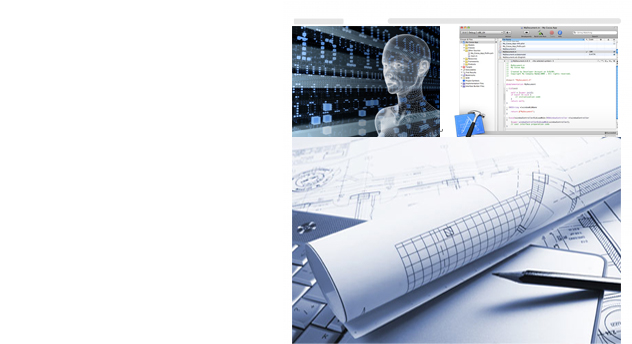
\includegraphics[width=1\textwidth]{../comon/figures/sddPic.jpg}
\cleardoublepage
\section{Introduction}
	\subsection{But du chapitre}
		Ce chapitre décrit les variantes d'architecture étudié pour le projet ESIP@PAD, l'architecture finale choisie ainsi que le détail du design final du projet. A l'aide de ce document il est possible de comprendre le fonctionnement technique de l'ensemble du projet.
	\subsection{Aperçu du chapitre}
	La section 2 contient l'architecture de notre système ainsi que les différentes alternatives possible. 
	
	La section 3 contient la description détaillée de l'implémentation de chaque composant du système ainsi que le détail concernant les algorithmes et techniques utilisés pour réaliser les parties majeure du système.

\section{Architecture du système }
	\subsection{Architecture choisie}	
		 \EPSFIGTEXTWIDTH{../comon/figures/GlobalArchitect.pdf}{Vue global de l'architecture du système}{archGlob}
		 Ce diagramme( Figure~\ref{archGlob}) nous donne un aperçu des différentes couche qui forment l'architecture du système.
		 
		 \textbf{View : } Cette couche du système sert a représenter graphiquement l'information. Elle est étroitement lié à la couche Controllers.\\[0.5cm]
		 \textbf{Controllers :} Cette couche du système s'occupe de charger les données dans la vue. Et de réagir correctement au événement reçu depuis l'utilisateur.\\[0.5cm]
		\textbf{Data Access Object:} Cette couche fait référence au pattern  de DAO \cite{daoMsc} qui nous permet d'accéder aux données de notre application sans se soucier d'où elles proviennent, d'où elles seront stockées ni comment. Elle contient aussi la logique métier de l'application. A l'aide de cette couche, il nous est facile de changer le support de stockage des données car toute la logique et l'accès au données y est centralisé. \\[0.5cm]
		\textbf{Core Data} est le frameworks de persistance de l'iOS qui permet d'accéder d'un manière simplifié au données stockées dans la base de données SQL-Lite ou sous format XML. Ce frameworks nous permet de décrire la base de données et ses relations et de générer des objets Objective-c qui correspondes aux entités de la base de données. Les principes du fonctionnement sont les mêmes que ceux du fameux framework JPA\cite{jpaNMSC} de java.


	\subsection{Discussion des alternatives d'architectures}
		Différentes alternatives d'architectures se sont offertes à nous en début du projet et voici les principales.
		
		\subsubsection{Alternative 1: Sans base de données }
		Cette alternative supprime la couche core data et la remplace par un stockage des données xml reçu des web-services sur le support de données de l'appareil. Cette alternative requière moins de temps de développement mais en contrepartie, il faut à chaque utilisation des données parser les fichiers xml. L'iOS n'est pas encore optimisé pour le traitement des fichiers xml et permet uniquement de parser un fichier mais sans faire des requêtes du type XPath sur les fichiers xml. Des frameworks ont été développés par divers entreprises pour permettre le requêtage de fichiers XML, mais leurs performances restent tout de même moins bonne que celle d'une base de données.
		
		\subsubsection{Alternative 2: Objet pour la communication en C++ }
		Cette alternative propose de décrire les objets pour la communication(Core data \begin{math} \Leftrightarrow \end{math} DAO  \begin{math} \Leftrightarrow \end{math} Controllers) en C++. Avec cette alternative, on augmente la portabilité de notre application et offre la possibilité de réutiliser ces mêmes objets sur d'autre plateforme (tel que Android). Après une bref recherche, il s'est avéré que Core data n'est pas capable d'utiliser les objet C++.. Comme nous utilisons une base de données SQL-Lite et que Core data génère automatiquement les objets correspondant  au contenu de la base de données nous avons mis de côtés cette alternative.  Par contre la base de données étant décrite en SQL-Lite, elle peut être exporter vers d'autre appareil et à partir de cette base de données il est facile de générer les objets de communication à l'aide des outils propre à chaque plateforme.
				
			 
	\subsection{Composants du système}
		\EPSFIGTEXTWIDTH{../comon/figures/ComposantSystem.pdf}{Diagrammes de composant du système}{ComposantSystem}
		L'application est découpée en composant pour ainsi permettre de bien séparer les tâches que l'on est entrain effectuée, facilité la réutilisation de partie de l'application et rendre les tests plus efficace vu que l'on ce concentre sur une partie et non pas un toute.

		Les composants n'ont pas été développé complètement dans le règle de l'art vu qu'on  n'a pas pour chaque composant un fichier compiler qui permet sa réutilisation ainsi qu'une interface pour y accéder(système de black-box). Cette entrave à la règle est dû au manque d'intérêt par l'obtention de composant si sophistiqué vu qu'il ne seront pas réutilisé en dehors de notre application et pour des raisons d'économie de temps. Mais cependant le code est organisé et conçu de manière à faciliter ça réutilisation dans un autre cadre et à pouvoir être transformé en composant complet(black-box) si besoin.
		
		\subsubsection{Description des composants}
		Voici une bref description des composants, le détail concernant leurs implémentation ce trouve dans la section suivante.
		\subsubsection*{Navigation:}
		Ce composant se charge de présenter un menu avec des boutons pour accéder aux composants de l'application. Lors d'un clique sur un des ses boutons, il est présenté à l'endroit approprié. Chaque composant appelé fera appel au composant ''Navigation'' pour être déchargé de la vue principale.
		\subsubsection*{Map:}
		Ce composant affiche une carte avec des indications sur les divers lieux de l'université. Il permet aussi de chercher l'emplacement d'une personnes ou d'une salle.
		\subsubsection*{Settings:}
		Ce composant permet de configurer les différents paramètres de l'application.
		\subsubsection*{News:}
		Ce composant permet d'afficher les news de l'université. Le détail des news est aussi affichable sous forme de page web intégré dans l'application et contenant le détail tel qu'il se trouve sur le site internet de l'USJ. 
		\subsubsection*{Calendrier:}
		Ce composant permet d'afficher pour chaque membre de l'université son emploi du temps. 
		\subsubsection*{ExamResult:}
		Ce composant permet aux étudiants d'afficher les résultats des examens
		\subsubsection*{Directory}
		Ce composant permet d'afficher l'annuaire de l'université. Il offre la possibilité d'envoyer des emails ou de lancer des appels à partir de l'application.




\section{Conception et Implémentation des composants}
	\subsection{Compatibilité graphique iPhone,iPad}
	Dès le lancement de l'iPad, Apple y a intégré un simulateur d'iPhone qui permet à toute application iPhone de s'exécuter sur l'iPad. 
			\begin{figure} [H]
				\centering 
				\subfigure[Apérçu de l'application FaceeBook vérsion iPhone executé sur iPad (zoom 1x) ]{\label{fig:gull}\includegraphics[width=0.4\textwidth]{../comon/figures/iPadCOmp1}} 
				\subfigure[Apérçu de l'édition d'un texte d'une applicaiton iPhone sur l'iPad (zoom 2x) ]{\label{fig:tiger}\includegraphics[width=0.4\textwidth]{../comon/figures/iPadCOmp2}} 
			\end{figure}
	Cette façon de faire peut être considéré comme une compatibilité, mais elle est minime vu qu'on étire simplement l'application iPhone pour la rendre plus grande mais on exploite nullement les capacités de l'écran de l'iPad.
	
	A la création d'un projet à l'aide de XCode, ce dernier nous demande si l'on veut créer une application iPhone, iPad ou universel. En choisissant universel, on s'attend à pouvoir faire une application pour un appareil et qu'elle soit compatible avec les 2. Mais l'illusion de cette compatibilité disparait assez vite. En effet pour la partie graphique il y a 2 dossiers , un nommé iPhone et l'autre iPad. Et là on comprend que la partie graphique doit être faite en grande partie à double. Ceci ne signifie pas que tout doit être fait à double, la plus part des composants ont leurs équivalents sur les 2 appareils. Les 2 composants uniquement disponible sur iPad sont le composant Split views et Popovers. 
	Dans une publication concernant\cite{appleComp} ce sujet  Apple  dit :\\
	
	 \textit{\textbf{Conditional Coding}\\
	In order to achieve your design goals for a Universal application, you will need to use conditional coding to determine the availability of features when your app is running. Conditional coding allows you to make sure you're loading the right resources, using functionality that's supported by the device and properly leveraging hardware that's available.}\\
	
	Et en effet tout au long du développement et pour les éléments que l'on désirer utiliser sur les 2 appareils sans duplication il a fallut tester pour savoir quel
	le code est exécuté et redimensionner les vues pour qu'elles soient à la bonne taille. 
	
	 Cette incompatibilité peut s'expliquer par la différence de taille des écrans, iPad: 241.2 mm x 185.7 mm et iPhone:115.2 mm x 58.6 mm. Et de plus l'information ne doit pas être organisé de la même façon sur les 2 appareils,sur iPad on pourra facilement présenter un plus grand nombres d'information sur un seul écran. Tandis que sur iPhone on doit essayer de minimiser l'information à afficher pour garantir qu'elle reste visible.
	 
	\subsection{Système de cache \label{sCache} }
		Un des points importants pour notre application est la mise en cache des données. Cette importance est dû à la vitesse de la connexion internet au Liban et de manière générale sur  tout les appareils mobiles. Ce manque de capacité des appareil mobile augmente le temps nécessaire pour accéder aux données. De plus même de nos jours, il n'est pas possible d'accéder à Internet de partout. 
		
		Pour le stockage en cache, un mécanisme de sauvegarde des dates d'exécution des requêtes a été mis en place. Pour chaque requête qu'on fait au serveurs 3 variables sont envoyé : le nom et password de l'utilisateur ainsi que le contenu qu'on désire obtenir. Dès l'exécution d'une requête la date de son exécution est enregistré, à la prochaine exécution si le temps écoulé entre la dernière exécution est aujourd'hui est supérieur à X(actuellement définit à 30 jours\footnote{Valeurs modifiable dans le fichier Settings.plist du code source}) on exécute à nouveau la requête sinon on récupère les valeurs du cache.

		\EPSFIGSCALE[0.4]{../comon/figures/algoCache}{Illustration du fonctionnement du système de cache. }{algoCache}
		
		Pour plus de détail à ce sujet, voir le code source de la  méthode areDataUpToDate de la classe GenericDAO ainsi que setLastUpdateTimeForKey et getLastUpdateTimeForKey de la classe  SettingsDAO.
		
	\subsection{Accès au données des services web}
	Le service informatique de l'université à mis en place un service web qui permet l'accès aux données  via le protocole HTTP et ils retourne essentiellement le contenu de la base de données sous format XML . Le service web se trouve actuellement à l'adresse: \url{http://www.usj.edu.lb/web-services/web-service.php}. Pour définir les données que l'on veut obtenir, on doit passer minimum par méthode post du protocol HTTP les paramètres suivant:
	\begin{enumerate}
	\item \textbf{usr} qui est le nom de l'utilisateur. guest est le nom par défaut et qui est valable pour les utilisateurs n'ayant pas de compte dans la base de données de l'USJ. Les autres utilisateurs doivent saisir leur id habituel pour les logins dans l'école. 
	\item \textbf{pwd} qui est le mot de passe de l'utilisateur. guest est le mot de passe pour les invités
	\item \textbf{op} est le nom de l'opération que l'on veut exécute. 	Voici la liste des opérations possible : 
	\begin{table}[H]
	\centering
	\begin{tabular}{|c|p{4cm}|p{7cm}|}
	\hline \textbf{Nom de l'opération }& \textbf{Description} & \textbf{paramètres}  \\ 
	\hline listeServRec & Renvoi la liste des services de l'USJ. & aucun \\ 
	\hline listeCampus & Renvoi la liste des camous de l'USJ. & aucun \\ 
	\hline listeInst & Renvoi la liste des institutions de l'USJ. & param0 = Code campus (optionnel) \\ 
	\hline listeEmpNom & Recherche la liste des employés de l'USJ d'après prénom et/ou nom. & param0 = Nom(optionnel)  param1= Prénom(optionnel). Au moins un paramètre est obligatoire  \\ 
	\hline listeEmpInst & Renvoi la liste des employés d'une institution de l'USJ. & param0 = Code Institution(obligatoire)   \\
	\hline listeEmpCampus & Renvoi la liste des employés d'un campus de l'USJ. & param0 = Code campus(obligatoire)  \\
	\hline listeBatiments & Renvoi la liste des bâtiments d'un campus de l'USJ. & param0 = Code campus(obligatoire)  \\
	\hline listeActualites & Renvoi les news de l'USJ. &aucun  \\
	\hline \color{red}listeHorraires & \color{red}Renvoi l'horaire d'une personne selon les données de login. & \color{red} Fonctionnalité uniquement implémenté sur les webServices en local.  \\
	\hline \color{red}listeNotes & \color{red}Renvoi les résultats d'examen d'une personne selon les données de login. & \color{red} Fonctionnalité uniquement implémenté sur les webServices en local.  \\
	\hline 
	\end{tabular} 
		\caption{Liste des opérations possible via les services web}
	\end{table}
	\end{enumerate}
	Une page internet \url{http://www.usj.edu.lb/web-services/send.php} permet de saisir les paramètres et de les exécuter pour tester les services web.
	
	Pour plus d'informations, concernant les web services, contacter M.Pascal TUFENKJ , Tel: +961 1 421 132 , Email: ptufenkji@usj.edu.lb
	
		\subsubsection{Services web locaux}
		Afin de minimiser la dépendance vis à vis des web services de l'USJ et de leur état d'avancement ,des web services locaux ont été créé. Leur fonctionnement est très simple c'est une simple page PHP hébergé sur la machine du développeur qui renvoie le fichier xml correspondant au nom de l'opération op. 
		
		Exemple : on envoi une requête http avec les parmètres en post suivant: usr=Elias, pwd=1234,op=listeNotes. Le fichier xml listeNotes.xml est retourné à l'utilisateur. 
		
		Pour plus d'informations, concernant les web services locaux voir le code source de la page webServices.php .

		\subsubsection{Téléchargement de fichier XML en Objective-c}
		Le téléchargement de données de grande tailles se fait de manière asynchrone à l'aide de la classe NSURLConnection. 
			\lstset{
			    style = Xcode,
			    caption=Téléchargement d'un fichier XML depuis internet de manière asynchrone et en transmettant les paramètres de la requête par POST .,
			    breaklines=true,
			    frame=single
			}
			
			\begin{lstlisting}[name= Loading data from internet in Objective-c, label=loadDataFromInternet]
-(void)loadDataFromInternet{

	// Initialise the request with the server url.
     NSMutableURLRequest *request = [NSMutableURLRequest requestWithURL:[NSURL URLWithString:@''http://serveurAdress.com/webServices.php'']   cachePolicy:NSURLRequestReloadIgnoringCacheData timeoutInterval:120.0]; 
   
    [request setHTTPMethod:@"POST"];  // Define the method of the request to Post
    
    NSString * postParam = [NSString stringWithFormat:@"usr=%@&pwd=%@&op=%@&param0=CST",  set.login,set.pasword,@"listEmpCampus"];
    // Post parm for getting the list of person of the CST campus
                 
    [request setHTTPBody:[webServicePostHeader dataUsingEncoding:NSASCIIStringEncoding]];
	// The delegate is self and self implement the 
    NSURLConnection *connection = [[[NSURLConnection alloc] initWithRequest:request delegate:self] autorelease]; 
    if (connection) { 
        receivedData = [[NSMutableData data] retain];
    } 
}

// this method is called for recieving every 256 byte of data
- (void)connection:(NSURLConnection *)connection didReceiveData:(NSData *)data {
    [receivedData appendData:data];
}
// this method will be called at the end of the connection (all data recieved)
- (void)connectionDidFinishLoading:(NSURLConnection *)connection{
	// Parse recieved XML file.
}
\end{lstlisting}
			\subsubsection{Exploiter des  XML en Objective-c}
			L'exploitation de fichiers XML se fait à l'aide du parser de l'iOS qui nous donne l'accès à l'information par événement (SAX).
			\lstset{
			    style = Xcode,
			    caption=Parsing d'un fichier XML en Objective-c .,
			    breaklines=true,
			    frame=single
			}
			
			\begin{lstlisting}[name= Parsing XML, label=NSXMLParser]
// receivedData is an  NSDATA object with row data of an XML file.
NSXMLParser *parseur=[[NSXMLParser alloc] initWithData:receivedData];
// Self is realising the NSXMLParserDelegate protocol
[parseur setDelegate: self];
// For the example the xml file is:
// <root>
//		<row>
//				<variable1>the value of variable 1 </variable1>
//				<variable2>the value of variable 2 </variable2>
//		</row>
//</root>
if([parseur parse] == NO){
	//Parsing error, mange it hier. 
}
[parseur release];	

//This method is called each time that an XML balise is opened
- (void)parser:(NSXMLParser *)parser didStartElement:(NSString *)elementName namespaceURI:(NSString *)namespaceURI qualifiedName:(NSString *)qName attributes:(NSDictionary *)attributeDict{
    if([elementName isEqualToString:@"row"]){// Create new object for getting data
		crntObject = [[NSObject alloc] init]
    }
    self.crntElementName =elementName;
}
//This method is called each time that a string (balise content) is found
- (void)parser:(NSXMLParser *)parser foundCharacters:(NSString *)string{
  
        NSString *newString = [[NSString alloc] initWithFormat:@"%@%@", crntCharacters,string];
        self.crntCharacters = newString;
        [crntObject setValue:newString forKey:self.crntElementName ];
        // We set the string value to the variable with the name of the current element
    }
}

//This method is called each time that an XML balise is closed
-(void)parser:(NSXMLParser *)parser didEndElement:(NSString *)elementName namespaceURI:(NSString *)namespaceURI qualifiedName:(NSString *)qName{
    if([elementName isEqualToString:@"row"]){// Close of the root element
        if (![crntObject save]) {
            NSLog(@'Whoops, couldn t save');
        }
    }
    
}
\end{lstlisting}

	\subsection{Base de donnée} 
	Pour stocké les données reçu depuis les services web, une base de données SQL-Lite est utilisé. La base de données est complètement géré par \gls{Core Data}. 
	La création des entités se fait dans \gls{XCode} en éditant le fichier ESIB\_PAD\_SOURCES.xcdatamodeld 
	\EPSFIGSCALE[0.6]{../comon/figures/dbCreate}{Interface dans X-Code permettant l'édition de la base de données}{dbCreate}
	
	Une fois les entités créé, édité il est possible de générer les objets correspondant aux entités à l'aide de la manipulation suivante: Sélectionné les entités   \begin{math} \Rightarrow \end{math} Dans le menu : Editor  \begin{math} \Rightarrow \end{math}  choisir Create NSMangedObject Subclass... 
	
	Une foie les objets correspondant aux entités sont généré, il est possible de les manipuler directement depuis le code. Dans notre application la manipulation des données se faits dans la couche DAO du système.
	
\lstset{
	style = Xcode,
	caption=Exemple de création  lecture et suppression de donnés dans la base à l'aide de Core Data .,
	breaklines=true,
	frame=single
}

\begin{lstlisting}[name=Create delete and read data, label=cd]
//Getting the managedObjectContext
// It's impotrant at the creation of the project to chooses application with support of Core Data to get acces to the  managedObjectContext  
NSManagedObjectContext * managedObjectContext =  [(ESIB\_PAD\_SOURCESAppDelegate *)[[UIApplication sharedApplication] delegate] managedObjectContext];

// Example: creating a new Campus in the DB.
NSManagedObject newObject = [NSManagedObject alloc];
newObject = [NSEntityDescription insertNewObjectForEntityForName:@'Campus' inManagedObjectContext:managedObjectContext];	
[newObject setValue:35.000 forKey:@'latitude'];
[newObject setValue:38.000 forKey:@'longitude'];
[newObject setValue:@'CST' forKey:@"code"];        
[newObject setValue:@'Rue de la paix 12' forKey:@"adresse"];
//... 
//...
[managedObjectContext save:\&error];// Persisting the new data.]


//Example: Reading list of person from campus CST
// The sql equivalent: SELECT * FROM Person where campus ='CST'

 NSFetchRequest * crntRequest = [[NSFetchRequest alloc] init];
NSEntityDescription *entity = [NSEntityDescription entityForName:self.entityDescription inManagedObjectContext:@'Person'];
[crntRequest setPredicate:[NSPredicate predicateWithFormat:@'campus = CST' ] ];// Filtering
[crntRequest setEntity:entity];
NSError *error;
NSArray *items = [managedObjectContext executeFetchRequest:crntRequest error:&error]; 

for (Person *p in items) {
    NSLog('User name is: %@', p.name);
}
[crntRequest release];


//Example: Deleting the campus CST from the DB
// The sql equivalent: Delete * from campus where code ='CST';

 NSFetchRequest * crntRequest = [[NSFetchRequest alloc] init];
NSEntityDescription *entity = [NSEntityDescription entityForName:self.entityDescription inManagedObjectContext:@'Campus'];
[crntRequest setPredicate:[NSPredicate predicateWithFormat:@'code = CST' ] ];// Filtering
[crntRequest setEntity:entity];
NSError *error;
NSArray *items = [self.managedObjectContext executeFetchRequest:crntRequest error:&error]; 

for (Person *p in items) {
        [managedObjectContext deleteObject:managedObject];
}
[managedObjectContext save:\&error];// Persisting the changement 
[crntRequest release];
\end{lstlisting}
	
	
	\subsection{Navigation}
		\subsubsection*{Diagramme de séquence}
			\EPSFIGTEXTWIDTH{../comon/figures/seqNavig.pdf}{Diagramme de séquence du principe de la navigation}{seqNavig}
			Le diagramme de séquence est valable pour les deux appareil la seul différence est que sur l'IPad la vue chargé  ne cachera pas l'écran entier mais rien qu'une partie de l'écran.
		\subsubsection*{Diagramme de classe}
			 \EPSFIGSCALE[0.7]{../comon/figures/ClasMainViewIPhone.pdf}{Diagramme de classe du composant MainView}{ClasMainViewIPhone}
		\subsubsection*{Discussion}
		Pour faciliter l'ajout ou suppression d'éléments dans le menu, ce dernier est créé automatiquement à partir  d'un fichier plist(Fichier xml de configuration pour l'iOS). 
			\EPSFIGSCALE[0.6]{../comon/figures/menuPlist}{Contenu du fichier MenuItemsParam.plist de configuration du menu pour la navigation}{menuPlist}
			
		L'accès en lecture et écriture aux données des fichier plist se fait très facilement comme ceci:
	\lstset{
	    style = Xcode,
	    caption=Code d'ecriture et de lecture dans un fichier plist.,
	    breaklines=true,
	    frame=single
	}
	
	\begin{lstlisting}[name=R/W in plist, label=SampleCode]
	// Wrinting value in Plist file
-(void)setValueForKey:(NSString *) theKey valure:(NSString *) value {
    NSArray *paths = NSSearchPathForDirectoriesInDomains( NSDocumentDirectory,
                                                         NSUserDomainMask, YES); 
    NSString *path =[[paths objectAtIndex: 0] stringByAppendingPathComponent: @"PlistFile.plist"];
    NSMutableDictionary * plistDict = [[NSMutableDictionary alloc] initWithContentsOfFile:path];
    if(!plistDict){
        plistDict = [[NSMutableDictionary alloc] init];
    }
    [plistDict setValue:value forKey:theKey];
    [plistDict writeToFile:path atomically: YES];
    [plistDict release];
}
	// Reading value form Plist file
-(NSString *)getValueForKey:(NSString *) theKey {
    NSString *docsDir = [NSSearchPathForDirectoriesInDomains(NSDocumentDirectory,NSUserDomainMask, YES) objectAtIndex:0];
    NSString *path = [docsDir stringByAppendingPathComponent: @"PlistFile.plist"];
    NSMutableDictionary* plistDict = [[NSMutableDictionary alloc] initWithContentsOfFile:path];
    NSString * d = [plistDict valueForKey:theKey];
    [plistDict autorelease];
    return  d;
}
\end{lstlisting}


		Suite à des problèmes d'affichage rencontré lors de la rotation des appareils, il a était décidé de centralisé la gestion de rotation des appareils dans cette partie de l'application. Pour se faire on va s'enregistrer pour recevoir les notifications de rotation et après chaque rotation, on va après chaque rotation redessiner l'interface en fonction de l'orientation. Une fois l'orientation de l'appareil détecté on va forcer le système à redessiner la vue comme on le désir. 
		
			\lstset{
			    style = Xcode,
			    caption=Code d'enregistrement pour la notification de rotation des appareils.,
			    breaklines=true,
			    frame=single
			}
		
			\begin{lstlisting}[name=Orientation did change notification  , label=SampleCode]
		//Registring for notification
[[NSNotificationCenter defaultCenter] addObserver:self selector:@selector(didRotate:) name:@"UIDeviceOrientationDidChangeNotification" object:nil];

- (void) didRotate:(NSNotification *)notification
{	
 UIInterfaceOrientation currentOrientation = [[UIDevice currentDevice] orientation];
    
    // Important: Somme times, the current device orientation is Unknown and then the only othe way to nows the orientation is the variable self.interfaceOrientation
    if (currentOrientation == UIDeviceOrientationUnknown ||
		currentOrientation == UIDeviceOrientationFaceUp ||
		currentOrientation == UIDeviceOrientationFaceDown){
		currentOrientation = self.interfaceOrientation;
    }
    if( UIDeviceOrientationIsLandscape(currentOrientation)){
		// Devise is in landscape redraw view for this orientation
	}else{
		// Devise is in portrait redraw view for this orientation
	}
}
		\end{lstlisting}
	\subsection{Settings}
		\subsubsection*{Diagramme de séquence}
			\EPSFIGTEXTWIDTH{../comon/figures/seqSettings.pdf}{Diagramme de séquence concernant la lécture et la modification des paramètres}{seqSettings}
			
		\subsubsection*{Diagramme de classe}
			 	\EPSFIGTEXTWIDTH{../comon/figures/ClassSettings.pdf}{Diagramme de classe du composant Settings}{ClassSettings}
		\subsubsection*{Discussion}

		Appel propose un système relativement simple pour modifier les paramètres d'une application. Ce système est capable d'à partir d'un fichier XML, créer l'interface graphique pour modifier son contenu. Le système d'appel \textbf{n'as pas été utilisé car il oblige l'utilisateur à sortir de l'application }et d'aller dans la fenêtre de paramétrage du système d'exploitation pour modifier les paramètres de l'application.  
		
		Le détail ainsi que l'utilité concernant les fonctions setLastUpdateTimeForKey et getLastUpdateTimeForKey est expliqué dans le chapitre~\ref{sCache}.

		
	\subsection{Map}
		\subsubsection*{Diagramme de séquence}
			\EPSFIGTEXTWIDTH{../comon/figures/seqCarte.pdf}{Exemple de séquence concernant l'affichage de la carte}{seqCarte}
			\EPSFIGTEXTWIDTH{../comon/figures/seqCarteSearch.pdf}{Exemple de séquence concernant la recherche d'un élément sur la carte}{seqCarteSearch}
			Le diagramme de séquence est valable pour les deux appareils la seul différence est que sur l'IPad la vue chargé  ne cachera pas l'écran entier mais rien qu'une partie de l'écran.
		\subsubsection*{Diagramme de classe}
			 	\EPSFIGTEXTWIDTH{../comon/figures/classCarte.pdf}{Diagramme de classe du composant Map}{classCarte}
		\subsubsection*{Discussion}
		\paragraph{Le framework MapKit }
		qui exploite les images de googleMap est utilisé pour afficher la carte. Son utilisation est simple et d'excellent tutoriel \cite{tutoNet} sur internet il est très facile de démarré avec cette librairie. Ce framework nous permet d'ajouter des indicateurs sur la carte pour signaler les emplacements intéressants. 


			\lstset{
			    style = Xcode,
			    caption=Code de création d'un objet MKMapView et l'ajout d'une annotation.,
			    breaklines=true,
			    frame=single
			}

\begin{lstlisting}[name=MapView with label  , label=MKMapView]
MKMapView * map = [[MKMapView alloc] initWithFrame:self.view.frame];

CLLocationCoordinate2D coordinate;
coordinate.latitude = 35.000;
coordinate.longitude = 33.000;            
MapLocations *annotation = [[[MapLocations alloc] initWithName:@"Un exemple d'annotation" description:@'"Voici une description" coordinate:coordinate] autorelease];
[map addAnnotation:annotation];
\end{lstlisting}
		Il est tout à fait pensable si par la suite on obtient des cartes des campus plus détaillées de les intégrer aux cartes existante. 
		
		\paragraph{L'appel asynchrone} nous permet de télécharger des données comme la liste de personnes ou l'emplacement des bâtiment depuis internet d'une manière transparente. Avec les appels asynchrone on évite que toute l'interface graphique soit gelé.
 		\EPSFIGTEXTWIDTH{../comon/figures/seqAsnyc.pdf}{Diagramme de séquence illustrant  l'appel asynchrone pour télécharger des données depuis internet}{seqAsnyc}


	\subsection{News}
			\subsubsection*{Diagramme de séquence}
				\EPSFIGTEXTWIDTH{../comon/figures/seqNews.pdf}{Exemple de séquence concernant l'affichage des news}{seqNews}
				Ce diagramme de séquence nous montre que les news sont de tout façon téléchargé depuis internet même si elles sont déjà en cache. Ce choix est dû à la nature des données qui doivent être toujours à jour. Cependant si il n'y a pas de connexion internet, les informations en caches seront tout de même affiché. 
			\subsubsection*{Diagramme de classe}
				 	\EPSFIGTEXTWIDTH{../comon/figures/ClassNews.pdf}{Diagramme de classe du composant News}{ClassNews}
			\subsubsection*{Discussion}
			
			
			\paragraph{Personnalisation des cellules d'un tableau:}Affin de rendre le design graphique plus attrayant, les cellules du tableau  ont été personnalisé. Il existe 2 principales façons pour modifier l'apparence des cellules:
		 	\begin{enumerate}
		 	\item La première consiste à modifier dans le code l'apparence avec des méthodes telle que setBackground, setColor. Cette méthode a un désavantage qui est de devoir exécuter la modification après chaque modification pour voir le résultat. De plus pour chaque cellule les mêmes opération seront refaites à chaque création.
		 	\item La deuxième solution est de crée un fichier NIB\footnote{http://fr.wikipedia.org/wiki/Interface\_Builder} à l'aide de l'outil graphique (Interface builder) inclus dans X-Code. Les avantages ici sont que l'on peut visuellement voir le résultat et on a une très grande liberté d'expression. De plus les objets sont directement stocké sous format binaire dans l'application et on doit pas pour chaque cellule perdre des ressources à les redessiner. L'inconvénient est que cette manière de faire nécessite plus de connaissance technique. 
		 	\end{enumerate}
			La deuxième variante a été utilisé et ainsi il est possible de personnalisé rapidement l'apparence des news.
			\EPSFIGTEXTWIDTH{../comon/figures/modifNewsCell.pdf}{Illustration de la modification de l'apparence des cellules et plus précisément la couleur du texte du titre.}{modifNewsCell}
			
			\paragraph{Téléchargement d'image à partir d'Internet} l'iOS offre la possibilité de loader des images depuis internet d'une manière simplifié. Mais le loading est fait d'une manière synchrone. Pour palier à ce problème nous pouvons utilisé la classe NSURLReques pour télécharger les données brut et de les traités en tant qu'image une fois toutes les données reçu. Pour plus de détail, voir le code source de la classe AsyncImageView dans le dossier Utility. 
			
	\subsection{Directory}
					\subsubsection*{Diagramme de séquence}
						\EPSFIGTEXTWIDTH{../comon/figures/seqAnnuaire.pdf}{Exemple de séquence concernant choix d'un filtre d'affichage et ensuite l'affichage d'une personne de l'annuaire}{seqAnnuaire}

					\subsubsection*{Diagramme de classe}
						 	\EPSFIGTEXTWIDTH{../comon/figures/classDirect.pdf}{Diagramme de classe du composant News}{classDirect}
					\subsubsection*{Discussion}
	
					\paragraph{Interface graphique sur iPad:} Il était prévu au départ d'utiliser un UISplitViewController qui permet d'avoir 2 parties, une pour naviguer et l'autre pour afficher le contenu. Mais après de longues heures  de recherche et d'essais, il s'avère que l'utilisation de se composant dans une partie de l'écran (et non en plein écran)n'est pas possible. De ce faite une interface qui répond à nos besoins a été conçu. Cette interface nous permet d'avoir un élément à droite pour l'affichage de contenu et à gauche une zone réservé pour la navigation. Les effets de transition on été fait à l'aide des fonctions d'animation de la classe UIView. 
	\lstset{
			    style = Xcode,
			    caption=Exemple de 2 animations à l'aide de la classe UIView. La première change la taille  et l'emplacement d'un élément graphique et la deuxième change sa transparence.,
			    breaklines=true,
			    frame=single
			}

\begin{lstlisting}[name=Animation UIView  , label=animateWithDuration]
-(void) animatteView:(UIView *) toAnim{
		// The first anim of the size to 50 x 50 and his position at x = 100 y =200;
        [UIView animateWithDuration:0.5 delay:0 options: UIViewAnimationCurveEaseOut
               animations:^{
                     CGRect rect = CGRectMake(100, 200, 50, 50);
                     toAnim.frame= rect;
                } 
                completion:^(BOOL finished){
					NSLog(@''First anim finish'')
                 }];
		// The second anim of the alpha value to 0 (transparent)
		// The delay proprietie help us to sync the animations
        [UIView animateWithDuration:0.5 delay:0.5 options: UIViewAnimationCurveEaseOut
               animations:^{
                     toAnim.alpha= 0;
                } 
                completion:^(BOOL finished){
					NSLog(@''Second anim finish'')
                 }];
    [UIView commitAnimations];// Starting the animation.

}
\end{lstlisting}

					Il aurait été intéressant d'avoir le temps pour rendre ce composant plus générique et de le publié sur internet pour ainsi éviter à d'autre utilisateurs de  devoir refaire le même travail.
					
					\paragraph{Recherche :}Pour offrir à l'utilisateur la fonction chercher, 2 méthode s'offre à nous
					\begin{enumerate}
					\item La première consiste à utilisé les requêtes SQL-Lite pour faire la recherche dans la base de données et d'afficher le résultat.
					\item La deuxième et de faire la recherche directement dans la liste de objet actuellement affiché et de masqué les éléments qui ne répondent pas au texte de recherche.
					\end{enumerate} 
					La deuxième façon est celle conseillé pas Apple. La première obligerai à chaque requête de réinitialiser chaque objet et serait trop couteuse en matière de ressources système. 
					
					Voici le code qui nous permet de filtrer les éléments dans la liste:
	\lstset{
			    style = Xcode,
			    caption=Methode de recherche dans une UITableView.,
			    breaklines=true,
			    frame=single
			}

\begin{lstlisting}[name=Recherche dans UITableView  , label=searchTBV]
- (void) searchTableView {
	NSString *searchText = searchBar.text;
	NSMutableArray *searchArray = [[NSMutableArray alloc] init];// Strings for searching
	
	// _persons is an array with the current displayed list 
	for (Person * p in _persons)
        {
        NSString  * s =  [NSString stringWithFormat:@" %@ %@ %@",p.nom , p.prenom ,p.carriere];
        // Whe want to search in the fileds : nom , prenom ,carriere
		[searchArray addObject:s];
        }
	int i=0;
	for (NSString *sTemp in searchArray)// We check each row
        {
        NSArray* separatedWord = [searchText componentsSeparatedByString: @" "];
        for (NSString *word in separatedWord) {
            NSRange titleResultsRange = [sTemp rangeOfString:word options:NSCaseInsensitiveSearch];
            if (titleResultsRange.length > 0){
                [copyListOfItems addObject:[_persons objectAtIndex:i]];
                break;
            }
        }
        i++;
     }
	[searchArray release];
	searchArray = nil;
	[self display:copyListOfItems];
}
\end{lstlisting}
					\paragraph{Lancer un appel téléphonique:} La philosophie d'Apple veut pour des raisons de sécurité garder chaque application dans son propre cadre et limiter la communication avec d'autre application. Cependant quelque tâche de base sont tout de même permis et l'une de celle là et de lancer un appel téléphonique depuis d'autre application. Mais une foie l'appel lancé, l'application est mise en background et elle ne sera pas remise au premier plan à la fin de l'appel. Cette contrainte est connu et elle est impossible de à contourné.
			\lstset{
				style = Xcode,
				caption=Lancement d'un appel téléphonique sur l'iPhone.,
				breaklines=true,
				frame=single
				}
					
\begin{lstlisting}[name=Recherche dans UITableView  , label=searchTBV]
- (void)calltoNum:(NSString  *)telNumber
{
        NSString *s  = [[NSString alloc] initWithFormat:@"tel://%@?",telNumber];
        [[UIApplication sharedApplication]openURL:[NSURL URLWithString:s]];   
        [s release];
}
\end{lstlisting}
					
			\paragraph{Écrire un e-mail:} On peut bien sur utilisé la même façon utilisé pour l'appel téléphonique ( remplacer tel:// par mailto ), mais il existe une autre variante plus élégante. Cette variante nous permet de rester dans l'application et d'éviter qu'à la fin de l'écriture de l'e-mail l'utilisateur doivent réouvrir l'application pour continuer son travail.  Le composant MFMailComposeViewController fournit avec l'iOS nous permet de faire ceci.
\lstset{
		style = Xcode,
		caption=Ouverture  de la fenêtre d'écriture d'e-mail,
		breaklines=true,
		frame=single
}
				
\begin{lstlisting}[name=Recherche dans UITableView  , label=searchTBV]
- (void)sendEmailTo:(NSString  *)destination
{
		if ([MFMailComposeViewController canSendMail]) {
            
            MFMailComposeViewController *mailComposer = [[MFMailComposeViewController alloc] init];
            [[mailComposer navigationBar] setTintColor:[UIColor colorWithRed:0.03f green:0.03f blue:0.03f alpha:1.0f]];
            mailComposer.mailComposeDelegate = self;
            [mailComposer setSubject:@"Subject"];
            [mailComposer setMessageBody:@"Sent from ESIB@PAD" isHTML:NO];
            [mailComposer setToRecipients:[NSArray arrayWithObject:destination]];
            [self presentModalViewController:mailComposer animated:YES];
            [mailComposer release];
        } else {
            UIApplication *app = [UIApplication sharedApplication];
            [app openURL:[NSURL URLWithString:
                          [NSString stringWithFormat:@"mailto:%@?subject=%@&body=%@",personInformation.email,@"Subject",@"Sent from ESIB@PAD"]]];
         }
}
\end{lstlisting}

	\subsection{Calendrier}
					\subsubsection*{Diagramme de séquence}
						\EPSFIGTEXTWIDTH{../comon/figures/seqCalendar.pdf}{Exemple de séquence concernant l'affichage de l'horaire pour une journée et l'affichage du détail de l'évènement sur la carte}{seqCalendar}

					\subsubsection*{Diagramme de classe}
						 	\EPSFIGSCALE[0.5]{../comon/figures/classCalendar.pdf}{Diagramme de classe du composant calendrier}{classCalendar}
						 	
					\subsubsection*{Discussion}
					\paragraph{GCCalendarPortraitView} est un composant Opensource téléchargé depuis internet et qui permet d'afficher une journée d'un calendrier avec des événements. Ce composant était de base uniquement compatible en mode plein écran sur IPhone et ne supporter pas la rotation de l'écran. Les modifications nécessaires ont été faites pour pouvoir l'utiliser dans une partie spécifique de l'écran(plus grand pour l'iPad). L'ajout de la possibilité de passer au jour suivant, précédent grâce au mouvement glisser du doigts a été aussi ajouter. 
\lstset{
		style = Xcode,
		caption=Enregistrement pour les notifications du mouvement glissement du doigt et réception de l'événement ,
		breaklines=true,
		frame=single
}
				
\begin{lstlisting}[name=Recherche dans UITableView  , label=searchTBV]
-(void) viewDidLoad{
    [super viewDidLoad];
    // Swipe Right notification
    UISwipeGestureRecognizer *swipeGesture = [[UISwipeGestureRecognizer alloc] initWithTarget:self action:@selector(swipe:)];
    swipeGesture.direction = UISwipeGestureRecognizerDirectionRight;
    [dayView addGestureRecognizer:swipeGesture];
    [swipeGesture release];
    
    // Swipe Left notification
    UISwipeGestureRecognizer *swipeGestureLeft = [[UISwipeGestureRecognizer alloc] initWithTarget:self action:@selector(swipe:)];
    swipeGestureLeft.direction = UISwipeGestureRecognizerDirectionLeft;
    [dayView addGestureRecognizer:swipeGestureLeft];
    [swipeGestureLeft release];
}
// Event sent when the  swipe mouvement is recognized.-
-(void)swipe:(UISwipeGestureRecognizer *)swipe{
    
    if(swipe.direction == UISwipeGestureRecognizerDirectionLeft){
        [self tomorow];
    }else if(swipe.direction == UISwipeGestureRecognizerDirectionRight){
        [self yesterday];   
    }
}
\end{lstlisting}
				\paragraph{Affichage de l'événement sur la carte}  Le même framework MapKit utilisé dans le composant Map est réutilisé ici pour afficher l'emplacement de l'événement sur la carte.

	\subsection{ExamResult}
					\subsubsection*{Diagramme de séquence}
						\EPSFIGTEXTWIDTH{../comon/figures/seqExamResult.pdf}{Exemple de séquence concernant l'affichage de l'horaire pour une journée et l'affichage du détail de l'évènement sur la carte}{seqExamResult}

					\subsubsection*{Diagramme de classe}
						 	\EPSFIGSCALE[0.5]{../comon/figures/classExamResult.pdf}{Diagramme de classe du composant calendrier}{classExamResult}
						 	
					\subsubsection*{Discussion}
					\paragraph{Tout comme les news}, si il y a une connexion internet, les données seront directement téléchargé depuis internet et non pas prise depuis le cache.

\cleardoublepage
\chapter{Software Test Description\label{std}}
\vspace{6cm}
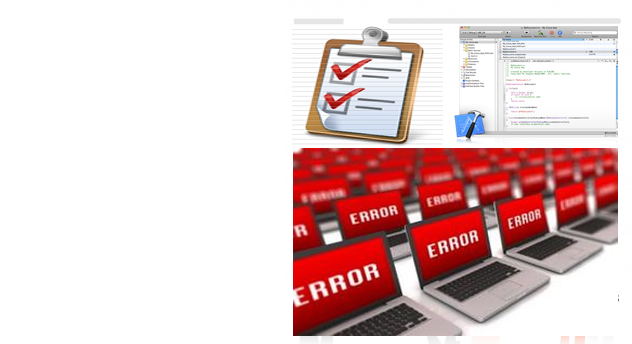
\includegraphics[width=1\textwidth]{../comon/figures/stdPic.jpg}
\cleardoublepage
\section{Introduction}
	Ce chapitre explique un partie importante d'un application qui est celle de test. La section cas de test décrit les  cas de test pour les tests de fonctionnalité. La partie protocole de test regroupe les protocoles de test qui ont été effectué après chaque release. 
	\subsection{Philosophie de test}
	\EPSFIGSCALE[1]{../comon/figures/testApercu.pdf}{Vue global de l'architecture du système}{archGlob}
	Les tests se feront sur trois niveaux, le premier niveau est celui des tests de fonctionnalités qui sont des tests fait par l'humain selon un procédés décrit dans la section ~\ref{tc}.  Le deuxième niveau est celui faits dans le code et qui sont reproductive automatiquement(Unit test).Le troisième niveau est celui des tests de fuite dans la mémoire(Memory Leaks), qui consiste à observer la mémoire lors de l'utilisation(cas d'utilisation chapitre~\ref{tc} ) de l'application et de vérifier qu'aucune variable est stocké en mémoire pour toujours.  Il est important d'indiquer que les cas de test sont imaginés en même temps que la spécification, ce qui nous permet d'avoir un point de référence concernant les objectif à atteindre. Voir le \gls{SPMP} chapitre ''Processus technique'' pour plus d'information.\\
	 A la fin de chaque itération, un protocole de test est rédigé après avoir tester les nouvelles fonctionnalités et retester les anciennes fonctionnalités. Grâce à cette stratégie, on est sûr que les nouvelles fonctionnalités n'empêche pas le fonctionnement des anciennes et que le toute reste compatible.
\section{Organisation des tests }
	\subsection{Éléments à tester}
		\begin{itemize}
			\item Le bon fonctionnements des différents cas d'utilisations
			\item Des tests unitaires pour la partie logique métier.
			\item Des analyses de fuites dans la mémoire(Leaks) doit être faite, vue que pour être visible sur l'appstore, une application ne doit pas contenir de Leaks.
		\end{itemize}
	\subsection{Éléments à ne pas tester}
		\begin{itemize}
			\item La sécurité des web services
			\item La cohérence des résultats retourné par les web services.
		\end{itemize}
	\subsection{Outils de test et environnement}
		Le framework OCUnit\footnote{\url{http://developer.apple.com/tools/unittest.html}} nous permet de faire d'écrire des tests unitaire. Son fonctionnement est assez proche de celui JUnit pour Java. Les fonctions tel que STAssertEqualObjects ou STAssertTrue permettent de faire échouer ou réussir un test.
		
		Pour le test des Memory Leaks l'outil Instruments\footnote{\url{http://developer.apple.com/library/mac/\#documentation/DeveloperTools/Conceptual/InstrumentsUserGuide}} qui est prévu à cet effet est utilisé. Depuis XCode, choisir 'Product \begin{math}
		\Rightarrow \end{math} Profile' pour exécuter à l'aide de Instruments. Une fois le code lancé choisir Leaks comme template de base. Ensuite utilisé l'application selon un cas de test. L'outil vous indiquera si des leaks existe et leurs emplacement.
		 
\section{Cas de test \label{tc}}
	\subsection{Navigation}
				 \begin{longtable}{m{4cm}|p{10cm}|}
				 \textbf{ ID} & 1 \\
				 \hline \textbf{Déscirption} & Test que l'on peut bien naviguer d'un vue à l'autre sans erreurs\\
				 \hline \textbf{Déroulement} &
					 \begin{itemize}
						 \item Fermer complètement l'application si elle était ouverte
						 \item Ouvrir l'application
						 \item  Pour chaque vue, cliquer sur le logo pour ouvrir, voir si le résultat obtenu est cohérent, revenir au menu principal.
						 \item  Pour chaque vue, cliquer sur le logo pour ouvrir, modifier le contenu dans la vue, fermer l'application à l'aide du bouton menu de l'appareil, réouvrir l'application, vérifie que c'est toujours cette vue qui est visible et qu'aucune information n'a été perdu après la manœuvre. 
						 \item  Pour chaque vue, cliquer sur le logo pour ouvrir. faire 4 x une rotation de 90 degrés à l'appareil. Vérifier qu'après chaque rotation la vue est dans le bon sens et que les éléments sont affiché correctement. 
					 \end{itemize}
				 \\
			 \end{longtable} 
	\subsection{Paramétrer}
			 \begin{longtable}{m{4cm}|p{10cm}|}
			 \textbf{ ID} & 2 \\
			 \hline \textbf{Déscirption} & Test que l'on peut modifier les paramètres de l'application\\
			 \hline \textbf{Déroulement} &
				 \begin{itemize}
					 \item Fermer complètement l'application si elle était ouverte.
					 \item Ouvrir l'application.
					 \item  Ouvrir la fenêtre de paramètres.
					 \item  Pour chaque champs:
						 \begin{enumerate}
						 	\item Éditer la valeurs.
						 	\item fermer la fenêtre de paramètres.
						 	\item Réouvrir la fenêtre de paramètres.
						 	\item Vérifier que les valeurs sont bien celle saisi auparavant.
						 \end{enumerate}
					 \item Modifier tout les paramètres.
					 \item Fermer complètement l'application(À l'aide du gestionnaire d'application et non seulement à l'aide du bouton menu. )
					 \item Réouvrir l'application et être sûr que les modifications ont bien été enregistré.
				 \end{itemize}
			 \\
		 \end{longtable} 
		\subsection{Carte}
					 \begin{longtable}{m{4cm}|p{10cm}|}
					 \textbf{ ID} & 3 \\
					 \hline \textbf{Déscirption} & Test du bon fonctionnement de la carte.\\
					 \hline \textbf{Déroulement} &
						 \begin{itemize}
						  	\item Se rendre au campus de l'ESIB
						  	\item Se connecter à internet
							 \item Fermer complètement l'application si elle était ouverte.
							 \item Ouvrir l'application.
							 \item Ouvrir la fenêtre de la carte.
							 \item Presser le bouton Localiser moi et vérifier que l'endroit retourné et au bon emplacement.
							 \item Vérifier que l'application afficher des indicateurs sur les principaux immeubles du campus.
							 \item Se déplacer dans  le campus est vérifier que l'indicateur de position actuelle suit le déplacement.
							\item Saisir le nom d'une personne dans la bar de recherche, vérifier qu'on obtient en suivants les écrans un indicateurs concernant l'emplacement du bureau de cette personne.
							\item Saisir le nom d'une classe dans la bar de recherche et faire de même que l'étape précédente.
							\item Saisir le nom d'un bâtiment dans la bar de recherche et faire de même que l'étape précédente.
							\item Pressez sur le bouton de Navigation par élément.
							\begin{itemize}
								\item Choisir: Bâtiments 
								\item Choisir un bâtiments  spécifique et vérifier que son emplacement est affiché sur la carte. 
							\end{itemize}
							\item Se déconnecter d'Internet et recommencer les étapes précédentes. Les mêmes fonctionnalités doivent être visible
						 \end{itemize}
					 \\
				 \end{longtable} 
				 
		\subsection{News}
					 \begin{longtable}{m{4cm}|p{10cm}|}
					 \textbf{ ID} & 4 \\
					 \hline \textbf{Déscirption} & Test du bon fonctionnement de l'affichage des news.\\
					 \hline \textbf{Déroulement} &
						 \begin{itemize}
						  	\item Installer à neuf l'application
						  	\item Se connecter à internet
							 \item Fermer complètement l'application si elle était ouverte.
							 \item Ouvrir l'application.
							 \item Ouvrir la fenêtre des news.
							 \item Comparer le résultat avec celui de la page internet:\url{http://www.usj.edu.lb/}
							 \item Visualiser le détail des news et vérifier que le détail correspond à la news.
							\item Se déconnecter d'Internet et recommencer les étapes précédentes. Les mêmes fonctionnalités doivent être visible
						 \end{itemize}
					 \\
				 \end{longtable} 

		\subsection{Directory}
					 \begin{longtable}{m{4cm}|p{10cm}|}
					 \textbf{ ID} & 5 \\
					 \hline \textbf{Déscirption} & Test du bon fonctionnement de l'annuaire.\\
					 \hline \textbf{Déroulement} &
						 \begin{itemize}
						  	\item Installer à neuf l'application
						  	\item Se connecter à internet
							 \item Fermer complètement l'application si elle était ouverte.
							 \item Ouvrir l'application.
							 \item Ouvrir la fenêtre de l'annuaire.
							 \item Choisir au moins 3 filtres d'affichages différents et s'assurer que les résultats sont bien cohérents. 
							 \item Choisir une personne et envoyer un e-mail via le lien mail.
							 \item Sur l'iPhone, cliquer sur le numéro de téléphone d'une personne et vérifier que l'appel est lancé.
							\item Se déconnecter d'Internet et recommencer les étapes précédentes. Les mêmes fonctionnalités doivent être visible
						 \end{itemize}
					 \\
				 \end{longtable} 
				 
		\subsection{Calendrier}
					 \begin{longtable}{m{4cm}|p{10cm}|}
					 \textbf{ ID} & 6 \\
					 \hline \textbf{Déscirption} & Test du bon fonctionnement de l'affichage du calendrier.\\
					 \hline \textbf{Déroulement} &
						 \begin{itemize}
						  	\item Installer à neuf l'application
						  	\item Se connecter à internet
							 \item Fermer complètement l'application si elle était ouverte.
							 \item Ouvrir l'application.
							 \item Paramétrer l'application pour obtenir les données depuis le web service local.
							 \item Ouvrir la fenêtre du calendrier.
							 \item Passez au jour suivant , précédent en faisant un mouvement de glisser sur le calendrier.
							 \item En cliquant sur un cours, la carte s'affiche , avec l'emplacement de dernier. 
							\item Se déconnecter d'Internet et recommencer les étapes précédentes. Les mêmes fonctionnalités doivent être visible
						 \end{itemize}
					 \\
				 \end{longtable}

		\subsection{Résultat d'examen}
					 \begin{longtable}{m{4cm}|p{10cm}|}
					 \textbf{ ID} & 6 \\
					 \hline \textbf{Déscirption} & Test du bon fonctionnement de l'affichage des résultats d'examens.\\
					 \hline \textbf{Déroulement} &
						 \begin{itemize}
						  	\item Installer à neuf l'application
						  	\item Se connecter à internet
							 \item Fermer complètement l'application si elle était ouverte.
							 \item Ouvrir l'application.
							 \item Paramétrer l'application pour obtenir les données depuis le web service local.
							 \item Ouvrir la fenêtre de résultat d'examen.
							 \item Vérifier que les résultats sont affiché correctement et que les notes sont bien celles obtenu lors de l'examen.
							\item Se déconnecter d'Internet et recommencer les étapes précédentes. Les mêmes fonctionnalités doivent être visible
						 \end{itemize}
					 \\
				 \end{longtable} 
\section{Protocole de test}
	Ce qu'on entend par protocole de test, c'est l'exécution de l'application en suivant pas à pas les étapes décrite dans le cas de test. En parallèle à cette exécution, les test de Leaks dans la mémoire sont effectué.
	Après chaque release, tout le protocole de test est répété pour garantir que les nouvelles fonctionnalités n'empêche pas le bon fonctionnement des anciennes.
	L'exécution des testes unitaire fait aussi partie du protocole de test et leurs  logs sont mentionnés ci dessous. 
		\subsection{Protocole de test 1}
		\textbf{Version testé:} 0.1 (\url{https://esibpad.googlecode.com/svn/tags/0.1}) \\
		\textbf{	Date du test :} 20/06/2011

		\subsubsection*{Cas de test : Navigation}
				 \begin{longtable}{m{4cm}|p{10cm}|}
				 \textbf{ ID} & 1 \\
				 \hline \textbf{Déscirption} & Test que l'on peut bien naviguer d'un vue à l'autre sans erreurs\\
				 \hline \textbf{Commentaires} &Il existe pour le moment qu'une seule page. \\
				 \hline Objectif  atteint & {\color{green} Complètement 100\% \CheckedBox } \\
				\hline Visa & Elias Medawar \\	
				 \\
			 \end{longtable} 
 		\subsubsection*{Cas de test : Paramétrer}
		 \begin{longtable}{m{4cm}|p{10cm}|}
		 \textbf{ ID} & 2 \\
		 \hline \textbf{Déscirption} & Test que l'on peut modifier les paramètres de l'application\\
		 \hline \textbf{Commentaires} & 
		 	 	 \begin{enumerate}
				  		\item La fonction retenir n'est pas encore implémenté correctement, les valeurs sont de toutes façon enregistré.
				  		\item La validité des champs n'est pas implémenté, les valeurs peuvent être incohérente.
				  		\item Les valeurs des champs ''Retenir et carte'' ne sont enregistrés qu'en cas de modification d'un autre champ de type texte
				  	\end{enumerate} \\
 				\hline Objectif atteint &  {\color{red}partiellement 75\% \XBox} \\
 				\hline Visa & Elias Medawar 	\\
		 \\
		 \end{longtable} 
		 \subsubsection*{Test unitaire}
		 \begin{lstlisting}[language=C,caption = Log des test unitaires]
Test Suite 'ESIB_PADTests' started at 2011-06-20 06:33:02 +0000
Test Case '-[ESIB_PADTests testSettings]' started.
 Testing the settings DAO
Test Case '-[ESIB_PADTests testSettings]' passed (0.003 seconds).
Test Suite 'ESIB_PADTests' finished at 2011-06-20 06:33:02 +0000.
Executed 1 test, with 0 failures (0 unexpected) in 0.003 (0.003) seconds
		 \end{lstlisting}
		Objectif atteint : {\color{green}Complètement 100 \% \CheckedBox}
		 \subsubsection*{Test de fuite dans la mémoire}
		 		 \EPSFIGTEXTWIDTH{../comon/figures/leeks_graph1.png}{Résultat de l'analyse des Leeks à l'aide d'Xcode}{leeks0.1}
		 Objectif atteint : {\color{green}Complètement 100 \% \CheckedBox}\\
		 On peut voir que le code ne contient aucune fuite de mémoire.
		 
		 
		\subsection{Protocole de test 2}
		 		\textbf{Version testé:} 0.2 (\url{https://github.com/eia-fr/ESIB_PAD/tree/0.2}) \\
		 		\textbf{	Date du test :} 05/07/2011
		 
		 		\subsubsection*{Cas de test : Navigation}
		 				 \begin{longtable}{m{4cm}|p{10cm}|}
		 				 \textbf{ ID} & 1 \\
		 				 \hline \textbf{Déscirption} & Test que l'on peut bien naviguer d'un vue à l'autre sans erreurs\\
		 				 \hline \textbf{Commentaires} &Lors du chargement des informations depuis internet, le logo loading n'est pas centrer quand l'iphone est en paysage. \\
		 				 \hline Objectif  atteint & {\color{green} Complètement 100\% \CheckedBox } \\
		 				\hline Visa & Elias Medawar \\	
		 				 \\
		 			 \end{longtable} 
		  		\subsubsection*{Cas de test : Paramétrer}
		 		 \begin{longtable}{m{4cm}|p{10cm}|}
		 		 \textbf{ ID} & 2 \\
		 		 \hline \textbf{Déscirption} & Test que l'on peut modifier les paramètres de l'application\\
		 		 \hline \textbf{Commentaires} & 
		 		 	 	 \begin{enumerate}
		 				  		\item La fonction retenir n'est pas encore implémenté correctement, les valeurs sont de toutes façon enregistré.
		 				  		\item La validité des champs est validé seulement au moment que les utiliser
		 				  		\item La carte est toujours en mode satellite.
		 				  	\end{enumerate} \\
		  				\hline Objectif atteint &  {\color{red}partiellement 85\% \XBox} \\
		  				\hline Visa & Elias Medawar 	\\
		 		 \\
		 		  \end{longtable} 		 		 
		 		 \subsubsection*{Cas de test : Carte}
		 		 		 \begin{longtable}{m{4cm}|p{10cm}|}
		 		 		 \textbf{ ID} & 3 \\
		 		 		 \hline \textbf{Déscirption} &  Test du bon fonctionnement de la carte.\\
		 		 		 \hline \textbf{Commentaires} &  
		 		 		 	 	 \begin{enumerate}
	 		 		 		 	 		\item La position de l'utilisateur est de toute façon affiché.
	 		 							\item Les coordonnées latitude longitude sont inversé pour les batiments du campus CTS
	 		 							\item {\color{red}L'application crache quand un campus n'as pas de bâtiment à afficher}.
	 		 		 		 	\end{enumerate} \\
	 		 		 		  				\hline Objectif atteint & {\color{orange} Partiellement 95\% \XBox } \\
	 		 		 		  				\hline Visa & Elias Medawar 	\\
		 		 		 \\
		 		 \end{longtable} 
		 		 \subsubsection*{Test unitaire}
		 		 \begin{lstlisting}[language=C,caption = Log des test unitaires]
Test Suite 'ESIB_PAD_SOURCESTests' started at 2011-07-05 07:37:38 +0000
Test Case '-[ESIB_PAD_SOURCESTests testCarte]' started.
 Testing the Campus DAO: You must uninstall the application before using this test
 Loading async the campus data from internet
 Waiting 30 sec for disabling the internet connection
 Getting campus data from cache?
 Comparing loacl and distant data
Test Case '-[ESIB_PAD_SOURCESTests testCarte]' passed (90.071 seconds).
Test Case '-[ESIB_PAD_SOURCESTests testSettings]' started.
 Testing the settings DAO
Test Case '-[ESIB_PAD_SOURCESTests testSettings]' passed (0.004 seconds).
Test Suite 'ESIB_PAD_SOURCESTests' finished at 2011-07-05 07:39:08 +0000.
Executed 2 tests, with 0 failures (0 unexpected) in 90.075 (90.077) seconds
		 		 \end{lstlisting}
		 		Objectif atteint : {\color{green}Complètement 100 \% \CheckedBox}\\
		 		\\
		 		Tester des appels de méthodes asynchrone n'est pas une tâche évidente. Notre calsse de test tourne dans le thread A et la class testé dans le thread B . Pour parvenir à faire cet opération on utilise les méthodes synchronisation mise à disposition de l'IOS pour bloquer le thread A durant le temps du téléchargement des données depuis internet du thread B. Pour recevoir les données, notre classe de test est définit comme délégué de la classe testé. Ansi quand le thread B reçoit et a traité les données il notifie le thread B du résultat obtenu.
		 		 \subsubsection*{Test de fuite dans la mémoire}
		 		 	%\EPSFIGTEXTWIDTH{../comon/figures/leeks_graph1.png}{Résultat de l'analyse des Leeks à l'aide d'Xcode}{leeks0.1}
		 		 Objectif atteint : {\color{red}partiellement 50 \% \CheckedBox}\\
		 		 Un problème avec la classe NSPredicate crée des Leek, selon la théorie le code n'en contient pas. Mais l'outil de mesure en détecte, des recherches plus approfondi pour trouver une solution seront refait pour trouver un solution
		 
		\subsection{Protocole de test 3}
		 		\textbf{Version testé:} 0.3 (\url{https://github.com/eia-fr/ESIB_PAD/tree/0.3.1}) \\
		 		\textbf{	Date du test :} 14/07/2011
		 
		 		\subsubsection*{Cas de test : Navigation}
		 				 \begin{longtable}{m{4cm}|p{10cm}|}
		 				 \textbf{ ID} & 1 \\
		 				 \hline \textbf{Déscirption} & Test que l'on peut bien naviguer d'un vue à l'autre sans erreurs\\
		 				 \hline \textbf{Commentaires} &Lors du chargement des informations depuis internet, le logo loading n'est pas centrer quand l'iPhone		 est en paysage. \\
		 				 \hline Objectif  atteint & {\color{green} Complètement 100\% \CheckedBox } \\
		 				\hline Visa & Elias Medawar \\	
		 				 \\
		 			 \end{longtable} 
		  		\subsubsection*{Cas de test : Paramétrer}
		 		 \begin{longtable}{m{4cm}|p{10cm}|}
		 		 \textbf{ ID} & 2 \\
		 		 \hline \textbf{Déscirption} & Test que l'on peut modifier les paramètres de l'application\\
		 		 \hline \textbf{Commentaires} & 
		 		 	 	 \begin{enumerate}
		 				  		\item La fonction retenir n'est pas encore implémenté correctement, les valeurs sont de toutes façon enregistré.
		 				  	\end{enumerate} \\
		  				\hline Objectif atteint &  {\color{orange}partiellement 95\% \XBox} \\
		  				\hline Visa & Elias Medawar 	\\
		 		 \\
		 		  \end{longtable} 		 		 
		 		 \subsubsection*{Cas de test : Carte}
		 		 		 \begin{longtable}{m{4cm}|p{10cm}|}
		 		 		 \textbf{ ID} & 3 \\
		 		 		 \hline \textbf{Déscirption} &  Test du bon fonctionnement de la carte.\\
		 		 		 \hline \textbf{Commentaires} &  
		 		 		 	 	 \begin{enumerate}
	 		 		 		 	 		\item La position de l'utilisateur est de toute façon affiché.
	 		 		 		 	\end{enumerate} \\
	 		 		 		  				\hline Objectif atteint & {\color{green} Complètement  100\% \CheckedBox } \\
	 		 		 		  				\hline Visa & Elias Medawar 	\\
		 		 		 \\
		 		 \end{longtable} 
		 		 \subsubsection*{Cas de test : News}
		 		 		 		 		 \begin{longtable}{m{4cm}|p{10cm}|}
		 		 		 		 		 \textbf{ ID} & 4 \\
		 		 		 		 		 \hline \textbf{Déscirption} &  Test du bon fonctionnement de la carte.\\
		 		 		 		 		 \hline \textbf{Commentaires} &  
		 		 		 		 		 	 	 \begin{enumerate}
		 		 	 		 		 		 	 		\item Les news ne sont pas toujours les mêmes que celle sur le site, apparemment les webservices ne fournissent qu'un partie des news pour l'application
		 		 	 		 					 	\end{enumerate} \\
		 		 	 		 		 		  				\hline Objectif atteint & {\color{green} Complètement 100\% \CheckedBox } \\
		 		 	 		 		 		  				\hline Visa & Elias Medawar 	\\
		 		 		 		 		 \\
		 		 		 		 \end{longtable} 
		 		 \subsubsection*{Test unitaire}
		 		 \begin{lstlisting}[language=C,caption = Log des test unitaires]
Test Suite 'ESIB_PAD_SOURCESTests' started at 2011-07-12 14:40:32 +0000
Test Case '-[ESIB_PAD_SOURCESTests testCarte]' started.
 Testing the Campus DAO: You must uninstall or reset cache of the application before testing
 Loading async the campus data from internet
 DATA recieved
Test Case '-[ESIB_PAD_SOURCESTests testCarte]' passed (60.564 seconds).
Test Case '-[ESIB_PAD_SOURCESTests testNews]' started.
 Testing the News DAO: You must uninstall or reset cache of the application before testing
 Loading async the news data from internet
 DATA recieved
Test Case '-[ESIB_PAD_SOURCESTests testNews]' passed (61.191 seconds).
Test Case '-[ESIB_PAD_SOURCESTests testSettings]' started.
Testing the settings DAO
Test Case '-[ESIB_PAD_SOURCESTests testSettings]' passed (0.073 seconds).
Test Suite 'ESIB_PAD_SOURCESTests' finished at 2011-07-12 14:42:34 +0000.
Executed 3 tests, with 0 failures (0 unexpected) in 121.828 (121.830) seconds
		 		 \end{lstlisting}
		 		Objectif atteint : {\color{green}Complètement 100 \% \CheckedBox}\\
		 		\\
		 		Le principe de teste de classe asynchrone décrit plus haut est réutilisé pour le test: testNews.
		 		 \subsubsection*{Test de fuite dans la mémoire}
		 		 \EPSFIGTEXTWIDTH{../comon/figures/leeks_graph1.png}{Résultat de l'analyse des Leeks à l'aide d'Xcode}{leeks0.1}
		 		 Objectif atteint : {\color{green}complètement 100 \% \CheckedBox}\\
	
	
	
		\subsection{Protocole de test 4}
		 		\textbf{Version testé:} 0.5 (\url{https://github.com/eia-fr/ESIB_PAD/tree/05}) \\
		 		\textbf{	Date du test :} 05/08/2011
		 
		 		\subsubsection*{Cas de test : Navigation}
		 				 \begin{longtable}{m{4cm}|p{10cm}|}
		 				 \textbf{ ID} & 1 \\
		 				 \hline \textbf{Déscirption} & Test que l'on peut bien naviguer d'un vue à l'autre sans erreurs\\
		 				 \hline \textbf{Commentaires} & Si on est entrain de loader des données depuis internet et que l'on choisis de passé à une autre fenêtre, l'application plante. \\
		 				 \hline Objectif  atteint & {\color{orange} Partiellement 95\% \CheckedBox } \\
		 				\hline Visa & Elias Medawar \\	
		 				 \\
		 			 \end{longtable} 
		  		\subsubsection*{Cas de test : Paramétrer}
		 		 \begin{longtable}{m{4cm}|p{10cm}|}
		 		 \textbf{ ID} & 2 \\
		 		 \hline \textbf{Déscirption} & Test que l'on peut modifier les paramètres de l'application\\
		  				\hline Objectif atteint &  {\color{green}Complètement 100\% \CheckedBox} \\
		  				\hline Visa & Elias Medawar 	\\
		 		 \\
		 		  \end{longtable} 		 		 
		 		 \subsubsection*{Cas de test : Carte}
		 		 		 \begin{longtable}{m{4cm}|p{10cm}|}
		 		 		 \textbf{ ID} & 3 \\
		 		 		 \hline \textbf{Déscirption} &  Test du bon fonctionnement de la carte.\\
		 		 		 \hline \textbf{Commentaires} &  
		 		 		 	 	 \begin{enumerate}
	 		 		 		 	 		\item La position de l'utilisateur est de toute façon affiché.
	 		 		 		 	\end{enumerate} \\
	 		 		 	\hline Objectif atteint & {\color{green} Complètement  100\% \CheckedBox } \\
	 		 		 	\hline Visa & Elias Medawar 	\\
		 		 		 \\
		 		 \end{longtable} 
		 		 \subsubsection*{Cas de test : News}
		 		 		 		 		 \begin{longtable}{m{4cm}|p{10cm}|}
		 		 		 		 		 \textbf{ ID} & 4 \\
		 		 		 		 		 \hline \textbf{Déscirption} &  Test du bon fonctionnement de la carte.\\
		 		 		 		 		 \hline \textbf{Commentaires} &  
		 		 		 		 		 	 	 \begin{enumerate}
		 		 	 		 		 		 	 		\item Les news ne sont pas toujours les mêmes que celle sur le site, apparemment les webservices ne fournissent qu'un partie des news pour l'application
		 		 	 		 					 	\end{enumerate} \\
		 		 	 		 		 		 \hline Objectif atteint & {\color{green} Complètement 100\% \CheckedBox } \\
		 		 	 		 		 		\hline Visa & Elias Medawar 	\\
		 		 		 		 		\\
		 		 		 		 \end{longtable} 
		 		 		 		 
		 		 \subsubsection*{Cas de test : Directory}
		 		 		 		 		 \begin{longtable}{m{4cm}|p{10cm}|}
		 		 		 		 		 \textbf{ ID} & 5 \\
		 		 		 		 		 \hline \textbf{Déscirption} &  Test du bon fonctionnement de l'annuaire.\\
		 		 		 		 		 \hline \textbf{Commentaires} &  
		 		 		 		 		 	 	 \begin{enumerate}
					 		 	 		 		 		 	 		\item Si on télécharge l'annuaire d'un Campus, et qu'après on désire avoir l'annuaire d'une institution(qui est une sous entité d'un campus) les informations de cette institution sont à nouveau téléchargé depuis internet. Ce qui signifie qu'on télécharge 2 fois les même information.
					 		 	 		 					 	\end{enumerate} \\
		 		 	 		 		 		 \hline Objectif atteint & {\color{orange} Partiellement 90\% \XBox } \\
					 		 	 		 		 		\hline Visa & Elias Medawar 	\\
					 		 		 		 		\\
		 		 		 		 \end{longtable}

		 		 \subsubsection*{Cas de test : Calendrier}
		 		 		 		 		 \begin{longtable}{m{4cm}|p{10cm}|}
		 		 		 		 		 \textbf{ ID} & 6 \\
		 		 		 		 		 \hline \textbf{Déscirption} &  Test du bon fonctionnement de la carte.\\
		 		 		 		 		 \hline \textbf{Commentaires} &  
		 		 		 		 		 	 	 \begin{enumerate}
					 		 	 		 		 		 	 		\item aucun bug détecté.
					 		 	 		 					 	\end{enumerate} \\
		 		 	 		 		 		 \hline Objectif atteint & {\color{green} Complètement 100\% \CheckedBox } \\
					 		 	 		 		 		\hline Visa & Elias Medawar 	\\
					 		 		 		 		\\
		 		 		 		 \end{longtable} 


		 		 \subsubsection*{Test unitaire}
		 		 \begin{lstlisting}[language=C,caption = Log des test unitaires]
Test Suite 'ESIB_PAD_SOURCESTests' started at 2011-08-07 12:48:23 +0000
Test Case '-[ESIB_PAD_SOURCESTests testCarte]' started.
  Testing the Campus DAO: You must uninstall or reset cache of the application before testing
  Loading async the campus data from internet
  Recievied async the Campus DATA
Test Case '-[ESIB_PAD_SOURCESTests testCarte]' passed (2.025 seconds).
Test Case '-[ESIB_PAD_SOURCESTests testDirectory]' started.
  Testing the Person DAO for the directory fonctionality: You must uninstall or reset cache of the application before testing
  Loading async the directory of the cmapus CST from internet
  List of person recieved
Test Case '-[ESIB_PAD_SOURCESTests testDirectory]' passed (17.585 seconds).
Test Case '-[ESIB_PAD_SOURCESTests testNews]' started.
  Testing the News DAO: You must uninstall or reset cache of the application before testing
  Loading async the news data from internet
  Recievied async the news DATA
Test Case '-[ESIB_PAD_SOURCESTests testNews]' passed (4.727 seconds).
Test Case '-[ESIB_PAD_SOURCESTests testPlaning]' started.
  Testing the Horraire DAO for the planning  fonctionality: You must uninstall or reset cache of the application before testing
  Loading async the plannong from internet
 Recievied async the planning from internet
Test Case '-[ESIB_PAD_SOURCESTests testPlaning]' passed (18.140 seconds).
Test Case '-[ESIB_PAD_SOURCESTests testSettings]' started.
 Testing the settings DAO
Test Case '-[ESIB_PAD_SOURCESTests testSettings]' passed (0.005 seconds).
Test Suite 'ESIB_PAD_SOURCESTests' finished at 2011-08-07 12:49:25 +0000.
Executed 5 tests, with 0 failures (0 unexpected) in 55.508 (55.538) seconds
		 		 \end{lstlisting}
		 		Objectif atteint : {\color{green}Complètement 100 \% \CheckedBox}\\
		 		\\
		 		Le principe de teste de classe asynchrone décrit plus haut est réutilisé pour les tests: testPlaning et testDirectory.
		 		 \subsubsection*{Test de fuite dans la mémoire}
		 		 \EPSFIGTEXTWIDTH{../comon/figures/leeks_graph1.png}{Résultat de l'analyse des Leeks à l'aide d'Xcode}{leeks0.1}
		 		 Objectif atteint : {\color{green}complètement 100 \% \CheckedBox}\\


		\subsection{Protocole de test 5}
		 		\textbf{Version testé:} 0.6 (\url{https://github.com/eia-fr/ESIB_PAD/tree/06}) \\
		 		\textbf{	Date du test :} 15/08/2011
		 
		 		\subsubsection*{Cas de test : Navigation}
		 				 \begin{longtable}{m{4cm}|p{10cm}|}
		 				 \textbf{ ID} & 1 \\
		 				 \hline \textbf{Déscirption} & Test que l'on peut bien naviguer d'un vue à l'autre sans erreurs\\
		 				 \hline \textbf{Commentaires} & Si on est entrain de loader des données depuis internet et que l'on choisis de passé à une autre fenêtre, l'application plante. \\
		 				 \hline Objectif  atteint & {\color{orange} Partiellement 95\% \CheckedBox } \\
		 				\hline Visa & Elias Medawar \\	
		 				 \\
		 			 \end{longtable} 
		  		\subsubsection*{Cas de test : Paramétrer}
		 		 \begin{longtable}{m{4cm}|p{10cm}|}
		 		 \textbf{ ID} & 2 \\
		 		 \hline \textbf{Déscirption} & Test que l'on peut modifier les paramètres de l'application\\
		  				\hline Objectif atteint &  {\color{green}Complètement 100\% \CheckedBox} \\
		  				\hline Visa & Elias Medawar 	\\
		 		 \\
		 		  \end{longtable} 		 		 
		 		 \subsubsection*{Cas de test : Carte}
		 		 		 \begin{longtable}{m{4cm}|p{10cm}|}
		 		 		 \textbf{ ID} & 3 \\
		 		 		 \hline \textbf{Déscirption} &  Test du bon fonctionnement de la carte.\\
		 		 		 \hline \textbf{Commentaires} &  
		 		 		 	 	 \begin{enumerate}
	 		 		 		 	 		\item La position de l'utilisateur est de toute façon affiché.
	 		 		 		 	\end{enumerate} \\
	 		 		 	\hline Objectif atteint & {\color{green} Complètement  100\% \CheckedBox } \\
	 		 		 	\hline Visa & Elias Medawar 	\\
		 		 		 \\
		 		 \end{longtable} 
		 		 \subsubsection*{Cas de test : News}
		 		 		 		 		 \begin{longtable}{m{4cm}|p{10cm}|}
		 		 		 		 		 \textbf{ ID} & 4 \\
		 		 		 		 		 \hline \textbf{Déscirption} &  Test du bon fonctionnement de la carte.\\
		 		 		 		 		 \hline \textbf{Commentaires} &  
		 		 		 		 		 	 	 \begin{enumerate}
		 		 	 		 		 		 	 		\item Les news ne sont pas toujours les mêmes que celle sur le site, apparemment les webservices ne fournissent qu'un partie des news pour l'application
		 		 	 		 					 	\end{enumerate} \\
		 		 	 		 		 		 \hline Objectif atteint & {\color{green} Complètement 100\% \CheckedBox } \\
		 		 	 		 		 		\hline Visa & Elias Medawar 	\\
		 		 		 		 		\\
		 		 		 		 \end{longtable} 
		 		 		 		 
		 		 \subsubsection*{Cas de test : Directory}
		 		 		 		 		 \begin{longtable}{m{4cm}|p{10cm}|}
		 		 		 		 		 \textbf{ ID} & 5 \\
		 		 		 		 		 \hline \textbf{Déscirption} &  Test du bon fonctionnement de l'annuaire.\\
		 		 		 		 		 \hline \textbf{Commentaires} &  
		 		 		 		 		 	 	 \begin{enumerate}
					 		 	 		 		 		 	 		\item Si on télécharge l'annuaire d'un Campus, et qu'après on désire avoir l'annuaire d'une institution(qui est une sous entité d'un campus) les informations de cette institution sont à nouveau téléchargé depuis internet. Ce qui signifie qu'on télécharge 2 fois les même information.
					 		 	 		 					 	\end{enumerate} \\
		 		 	 		 		 		 \hline Objectif atteint & {\color{orange} Partiellement 90\% \XBox } \\
					 		 	 		 		 		\hline Visa & Elias Medawar 	\\
					 		 		 		 		\\
		 		 		 		 \end{longtable}

		 		 \subsubsection*{Cas de test : Calendrier}
		 		 		 		 		 \begin{longtable}{m{4cm}|p{10cm}|}
		 		 		 		 		 \textbf{ ID} & 6 \\
		 		 		 		 		 \hline \textbf{Déscirption} &  Test du bon fonctionnement de la carte.\\
		 		 		 		 		 \hline \textbf{Commentaires} &  
		 		 		 		 		 	 	 \begin{enumerate}
					 		 	 		 		 		 	 		\item aucun bug détecté.
					 		 	 		 					 	\end{enumerate} \\
		 		 	 		 		 		 \hline Objectif atteint & {\color{green} Complètement 100\% \CheckedBox } \\
					 		 	 		 		 		\hline Visa & Elias Medawar 	\\
					 		 		 		 		\\
		 		 		 		 \end{longtable} 


		 		 \subsubsection*{Test unitaire}
		 		 \begin{lstlisting}[language=C,caption = Log des test unitaires]
Test Suite 'ESIB_PAD_SOURCESTests' started at 2011-08-07 12:48:23 +0000
Test Case '-[ESIB_PAD_SOURCESTests testCarte]' started.
  Testing the Campus DAO: You must uninstall or reset cache of the application before testing
  Loading async the campus data from internet
  Recievied async the Campus DATA
Test Case '-[ESIB_PAD_SOURCESTests testCarte]' passed (2.025 seconds).
Test Case '-[ESIB_PAD_SOURCESTests testDirectory]' started.
  Testing the Person DAO for the directory fonctionality: You must uninstall or reset cache of the application before testing
  Loading async the directory of the cmapus CST from internet
  List of person recieved
Test Case '-[ESIB_PAD_SOURCESTests testDirectory]' passed (17.585 seconds).
Test Case '-[ESIB_PAD_SOURCESTests testNews]' started.
  Testing the News DAO: You must uninstall or reset cache of the application before testing
  Loading async the news data from internet
  Recievied async the news DATA
Test Case '-[ESIB_PAD_SOURCESTests testNews]' passed (4.727 seconds).
Test Case '-[ESIB_PAD_SOURCESTests testPlaning]' started.
  Testing the Horraire DAO for the planning  fonctionality: You must uninstall or reset cache of the application before testing
  Loading async the plannong from internet
 Recievied async the planning from internet
Test Case '-[ESIB_PAD_SOURCESTests testPlaning]' passed (18.140 seconds).
Test Case '-[ESIB_PAD_SOURCESTests testSettings]' started.
 Testing the settings DAO
Test Case '-[ESIB_PAD_SOURCESTests testSettings]' passed (0.005 seconds).
Test Suite 'ESIB_PAD_SOURCESTests' finished at 2011-08-07 12:49:25 +0000.
Executed 5 tests, with 0 failures (0 unexpected) in 55.508 (55.538) seconds
		 		 \end{lstlisting}
		 		Objectif atteint : {\color{green}Complètement 100 \% \CheckedBox}\\
		 		\\
		 		Le principe de teste de classe asynchrone décrit plus haut est réutilisé pour les tests: testPlaning et testDirectory.
		 		 \subsubsection*{Test de fuite dans la mémoire}
		 		 \EPSFIGTEXTWIDTH{../comon/figures/leeks_graph1.png}{Résultat de l'analyse des Leaks à l'aide d'Xcode}{leeks0.1}
		 		 Objectif atteint : {\color{green}complètement 100 \% \CheckedBox}\\

\cleardoublepage
\chapter{Conclusion}
\cleardoublepage
\section{Évolutions futures}
Le résultat obtenu est un prototype fonctionnel est prête à être déployer. Cependant plusieurs fonctions peuvent venir le compléter pour le faire évoluer.
Voici les principales évolutions possible 
\subsection{Accès à toutes les données via les services web }  
Pour l'instant la base de données contient moins d'information que ce que l'application supporte. Les coordonnées GPS des bureau de personnes ainsi que ceux des salles de cours n'a pas été faite. Le planning de chaque personne ainsi que le résultat des examens ne sont pas encore accessible.
Cette évolution vise plus le côté services web de l'application mais qui est essentiel pour la suite de ce projet.

\subsection{Nouvelles fonctionnalités } 
Les idées de fonctionnalités supplémentaire proposées dans le cahier des charges peuvent compléter se projet. Les idées les plus intéressante serait:
\begin{enumerate}
\item La fonction ''Où es-tu?'' qui permet d'envoyer un message à une personne et si la personne le désire, ces coordonnés GPS seront renvoyé.  
\item Modification du calendrier. Permettre la modification(ajout/suppression/modification) d'événements dans le calendrier.
\end{enumerate}

\subsection{Version de l'application sur d'autre appareil}
D'autre appareil mobile ont les mêmes capacités que l'iPhone et l'iPad. Il serait aussi intéressant de rendre ce projet compatible avec les autres appareils. 

\subsection{Une version multilingue du projet.}
\subsection{Des cartes plus complètent des campus}
L'idée et de fournir des cartes plus détaillés des campus avec des plans détaillés des étages. Ces plans complèterait la carte actuelle de google map. 

\subsection{Accessible pour d'autre université}
Beaucoup d'autre université ont le besoin du même genres de fonctionnalités. L'idée ici est d'offrir la possibilité à d'autre université d'utiliser cette application mais avec leurs propres service web pour la gestion des données.

\section{Impressions personnelles} 
Pour moi ce projet représente pas uniquement le travail de 3 mois mais plutôt le résultat de 3 ans d'études passionnante. Mon principale but était d'appliquer le plus grand nombre de concept vu lors de mes études d'une façon exemplaire. Ce but est pour moi atteints et je suis satisfaits de mon travail.  Ce travail m'a permis de consolider la rampe  qui me servira pour le départ dans la vie actif et le monde de travail de l'ingénierie.  
   
C'est avec grand plaisir que j'ai était confronter au mode de travail de l'USJ au Liban. J'ai trouvé que le mode de travail à l'USJ est plus orienté résultat que celui auquel j'ai était confronté jusqu'à présent (à l'école ou lors d'autre expérience de travail). En ce sens je considère ce mode de travail plus proche de celui qui m'attend dans l'industrie. 

Le seul point négatif est qu'il n'a pas toujours était évident de garder une motivation constante tout au long du projet. Ceci est du à la durée(3 mois) de travail seul sur un projet.

J'ai pu traiter d'une manière assez profonde différent concept de développement iOS et peut me considérer désormais comme jeune connaisseur dans ce domaine.
C'est avec un petit chagrin au coeur que je termine ce projet passionnant  car il reste des choses intéressante à y développer. 

\section{Remerciements}
Je tiens à remercier M. Dany Mezher  en tant que responsable externe qui m'a suivi tout au long de ce travail.Il m'a soutenu autant sur le plan technique avec ses conseils d'expert dans le domaine du développement iOS que sur le plan social en m'accueillant généreusement et chaleureusement au Liban. J'espère que cette application pourra être utile à l'USJ. 

Je remercie aussi mes deux responsables internes, Mme Elena Mugellini et M. Omar Abou Khaled qui eux aussi m'ont suivi tout au long de mon travail.
Je remercie encore une fois M. Omar Abou Khaled  qui a organisé et rendu possible cette échange au Liban. 

Je remercie également mes deux experts, M. Marc Wuergle et M.Roland Marro.

Je remercie Mme Caroline Geissbühler pour la correction du rapport. Et plus particulièrement pour son soutient tout au long du projet. 

Pour terminer un merci particulier revient à ma famille au Liban qui m'ont accueillis et soutenu ainsi rendant ces 3 mois de séjour au Liban plus agréable .

\section{Conclusion}
Je m'attendais à une plus grand compatibilité entre l'iPhone et l'iPad et en conséquence a passé moins de temps sur la partie implémentation de chaque itération.

La méthodologie de travail itérative a permis de garantir une bonne  qualité du produit final. J'ai pu constater en découpant le temps à disposition en itération l'utilité d'avoir des jalons et de fixer des objectifs intermédiaire. 

Les objectifs fixé au départ du projet ont été atteint. Le prototype rendu est fonctionnel, il peut être facilement finalisé et exploité.  La documentation rendu avec le projet facilite la réutilisation et la continuation du projet  par une autre personne. Le code rendu est commenté et peut être aisément retravaillé pas d'autre personnes.

\cleardoublepage


\chapter{Indexes}
\cleardoublepage

\renewcommand{\bibname}{Références}

\begin{flushleft}
\bibliography{../comon/bibliography/references}
\end{flushleft}

\bibliographystyle{plain}


\printglossaries

\listoffigures

\lstlistoflistings

\cleardoublepage
\chapter{Annexes}
\section{Imprimé}
\subsection{Annexe A - directive du projet}
Contient la directive distribué au début du projet.
\subsection {Annexe F \- Flyer}
Le résumé du projet en allemand.
\subsection {Annexe G \- Cahier des charges}
Contient le cahier des charges établi au début du projet.
\subsection {Annexe H \- Journal de bord}
Le journal de bord.

\section{le CD}
 |- CodeSource : Contient tout les resources nécessaire pour le développement à l'aide de XCode\\
 |---AppDevCenterCertification : Contient les fichiers permettant d'accéder au compte développeur de l'EIF \\
 |---ESIB\_PAD\_SOURCES : Code source de l'application \\
 |-----ESIB\_PAD\_SOURCES : \\
 |-------Components : Contient les différents composant développé. La parite DAO de chaque composant est dans le dossier  DAO \\
 |---------Calendrier : Composant Calendrier\\
 |---------Directory : Composant Directory\\
 |-----------iPad : Partie graphique concernant l'iPAD\\
 |-----------iPhone : Partie graphique concernant l'iPone \\
 |---------ExamResult : Composant qui affiche les résultats de examens.\\
 |---------Map : Composant Map\\
 |---------Navigation: Composant Navigation avec le menu.\\
 |---------News : Composant News \\
 |---------Settings: Composant qui perment le paramétrage de l'application\\
 |-----------iPad : Partie graphique concernant l'iPAD\\
 |-----------iPhone : Partie graphique concernant l'iPone\\
 |---------Utility : Dossier contenant des classes à but d'utilitaire utilisé et développé dans le projet \\
 |-----------GCCalendar : version modifié du composant https://github.com/fraca7/GCCalendar/ \\
 |-------CoreDataEntities : Contient les entités de la base de données(Classe représentant une table dans la DB)\\
 |-------DAO : Contient toute les classe qui regroupe la logique métier et permet l'accès au donné.\\
 |-------ESIB\_PAD\_SOURCES.xcdatamodeld : Contient le modèl de la base de données \\
 |-------Images : Contient toutes les images, logo utilisé par l'application.\\
 |-----ESIB\_PAD\_SOURCESTests : Contient le code de test de l'application\\
 |---desing : Contient les fichiers Photoshop CS5 de design de l'application\\
 |---webServices : Contient le service web local écrit en php ainsi que les données.\\
 |-Documentation : Contient la documentation sous format PDF ainsi que le code Latex. \\
 |--- makeRapportFinal, make : sont des fichier bash permettant de générer la documentation (Compatible MAC OS X)\\
 |---Annexes\\
 |-----A\_Directive\\
 |-----B\_Plannigs\\
 |-----C\_ProcesVerbaux\\
 |-----D\_DiagramesUML\\
 |-----E\_XML\_WEB\_SERVICES\\
 |-----F\_Flyer\\
 |-----G\_Cahie\_des\_charges\\
 |-----H\_Journal\_de\_bord
 |---Source : Code latex pour la génération de la documentation\\
 |-----CDC : Cahier des charges\\
 |-----RapportFinal : Le rapport final.\\
 |-----RapportRelease : Les différent rapport de release.\\
 |-----SDD \\
 |-----SPMP\\
 |-----SRS\\
 |-----STD\\
 |-----comon\\
 |-------figure : Contient toute les figures et images utilisé dans la documentation.\\
 |-------logos : Les logos utilisé\\



\cleardoublepage
\chapter*{Annexe A \- Directives du projet}
\cleardoublepage
\chapter*{Annexe F \- Flyer}
\cleardoublepage
\chapter*{Annexe G \- Cahier des charges}

\cleardoublepage
\chapter*{Annexe H \- Journal de bord}

%\renewcommand{\bibname}{Referenzen}

%\begin{flushleft}
%\bibliography{./bibliography/references}
%\end{flushleft}

%\bibliographystyle{plain}




\end{document}
